\section{脂肪酸甲酯在H-ZSM-5分子筛上的吸附}
\par{通过传统的实验方法来获得吸附性质的效率很低,尤其是在反应的条件下研究长链分子的吸附更加困难。更重要的是,即使在温和的条件下,对于小分子而言,想通过实验的手段获得吸附位和吸附质构象等信息也是非常困难\cite{van1998chain}。}
\par{所以本章采用上文中构建的模型,使用Sorption模块,进行了丁酸甲酯、丁烯酸甲酯、油酸甲酯和反油酸甲酯在微介孔H-ZSM-5分子筛上的巨正则蒙特卡洛模拟(GCMC),考察了各类吸附分子在H-ZSM-5分子筛上的吸附性能,分析吸附分子链长和不饱和度、分子筛孔径和外界温度压力对于吸附性能的影响。}
\subsection{Sorption 参数设置}\label{Sorption 参数设置}
\par{本节使用Sorption模块进行吸附模拟,相关参数设置如下:}
\begin{enumerate}
    \item 任务选择:固定压力(Fixed pressure);温度设定:623K、673K、723K和773K(催化裂化反应温度);压力范围:0-500kPa内取点;平衡计算步数5000000步,生产步数10000000步;勾选返回最低能量构架(Return lowest energy frames),数量为10。
    \item 计算方法:Metropolis方法;精度选择:Ultra-fine。
    \item 力场选择:COMPASS\uppercase\expandafter{\romannumeral2};电荷选择:Use current。
    \item 加和方法中的静电相互作用选择埃瓦德方法(Ewald \& Group),非键相互作用选择原子基准(Atom based),非键截断值设置为18.5Å(正好小于晶胞最小边长一半)。
\end{enumerate}
\subsection{模型验证}\label{checking}
\par{为了验证本文计算采用的参数的正确性,本文将模拟计算出来的油酸甲酯和反油酸甲酯在微孔H-ZSM-5分子筛中的吸附结果与文献\cite{philippaerts2010selectivity}的实验结果相对比,模拟参数参照上文的参数设置,温度为室温25℃。对比结果如\reftab{tab:C18}所示。}


\begin{table}[H]
    \centering
    \caption{油酸甲酯与反油酸甲酯在H-ZSM-5分子筛内的吸附情况对比表}
    \begin{tabular}{p{2.5cm}<{\centering}p{2.5cm}<{\centering}p{2.5cm}<{\centering}p{2.5cm}<{\centering}p{2.5cm}<{\centering}}
        \toprule
        项目&硅铝比&$K_{ME}$&$K_{MO}$&$\alpha$\\
        \midrule
        实验&40&3.23&3.08&1.05\\
        模拟&36&2.92&2.63&1.02\\
		\bottomrule
    \end{tabular}
	\label{tab:C18}
\end{table}

\par{其中:$K_{ME}$表示反油酸甲酯的平衡吸附常数;$K_{MO}$表示油酸甲酯的平衡吸附常数;$\alpha$表示油酸甲酯与反油酸甲酯饱和吸附量的比值。由\reftab{tab:C18}可知,模拟与实验结果非常接近,误差不超过15\%,所以 \ref{Sorption 参数设置} 的参数设置是合理的。}

\subsection{模拟结果}
\subsubsection{吸附等温线}\label{吸附等温线}
\par{本小节按照 \ref{Sorption 参数设置} 的参数设置,首先计算了模型化合物丁酸甲酯和丁烯酸甲酯在微介孔H-ZSM-5分子筛,0~500kPa的吸附等温线,结果如\reffig{fig:sA}所示。}

\begin{figure}[H]
    \centering

    \subfigure[丁酸甲酯在微孔]{
    \begin{minipage}[t]{0.5\linewidth}
    \centering
    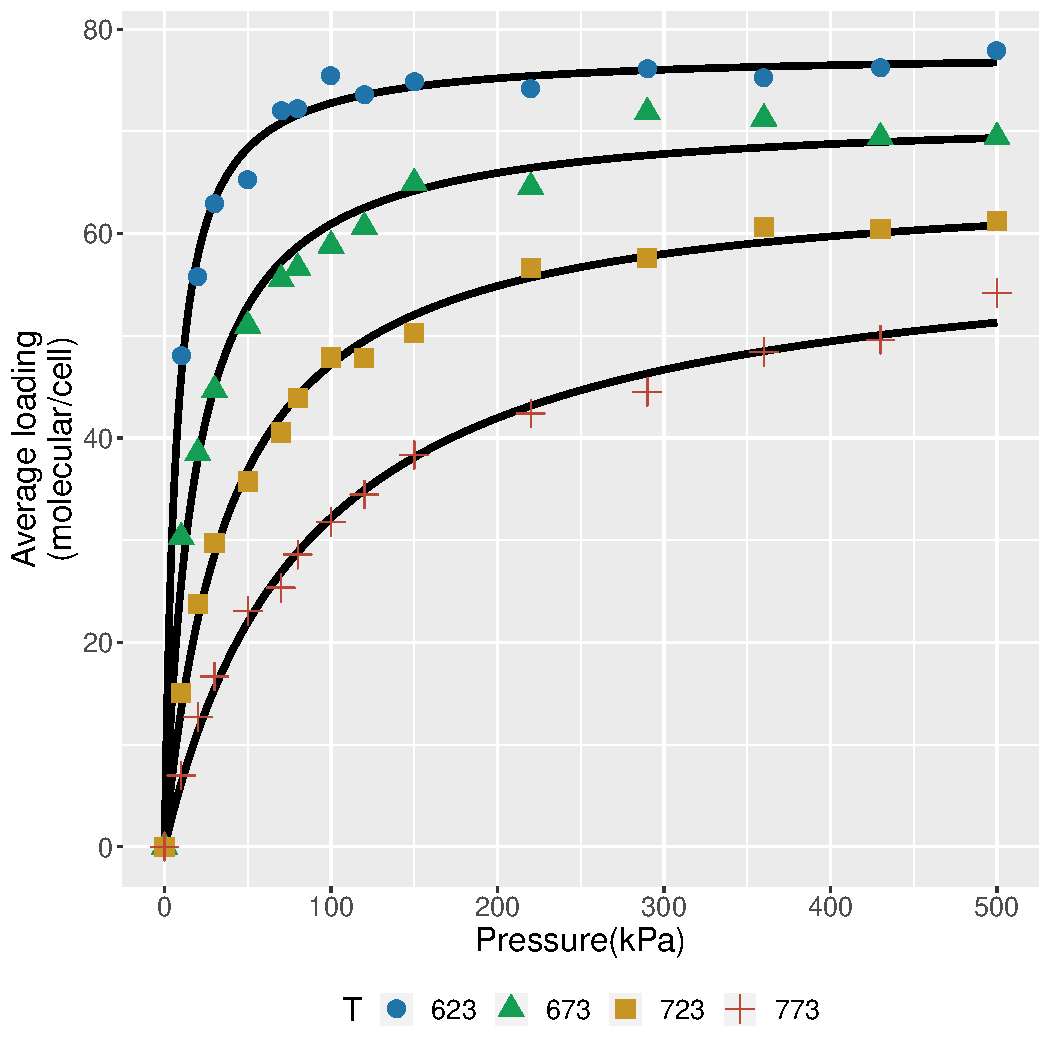
\includegraphics[width=2.7in]{figure/Adsorption/MicroPoreA.pdf}
    %\caption{fig1}
    \end{minipage}%
    }%
    \subfigure[丁烯酸甲酯在微孔]{
    \begin{minipage}[t]{0.5\linewidth}
    \centering
    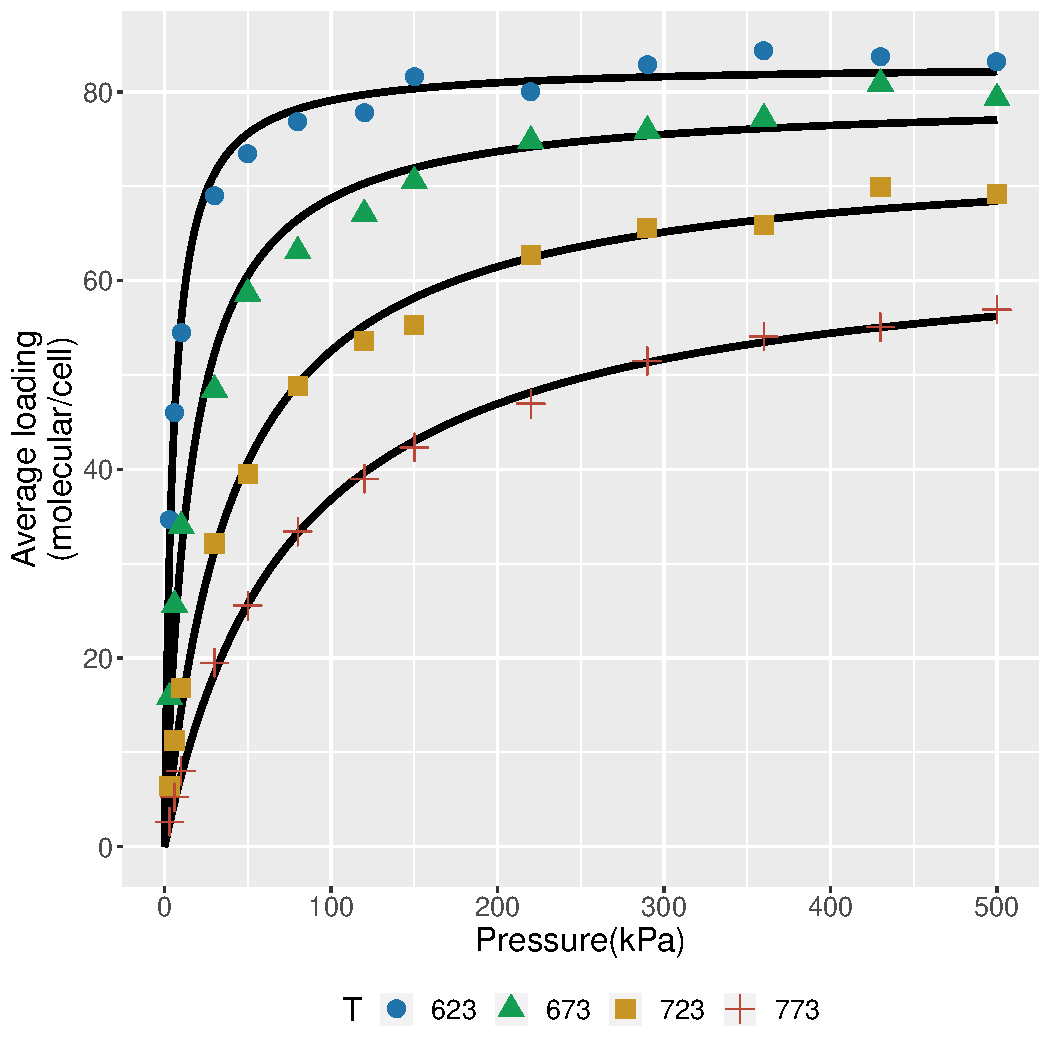
\includegraphics[width=2.7in]{figure/Adsorption/MicroPoreAunsaturated.pdf}
    %\caption{fig2}
    \end{minipage}%
    }%

    \subfigure[丁酸甲酯在20Å介孔]{
    \begin{minipage}[t]{0.5\linewidth}
    \centering
    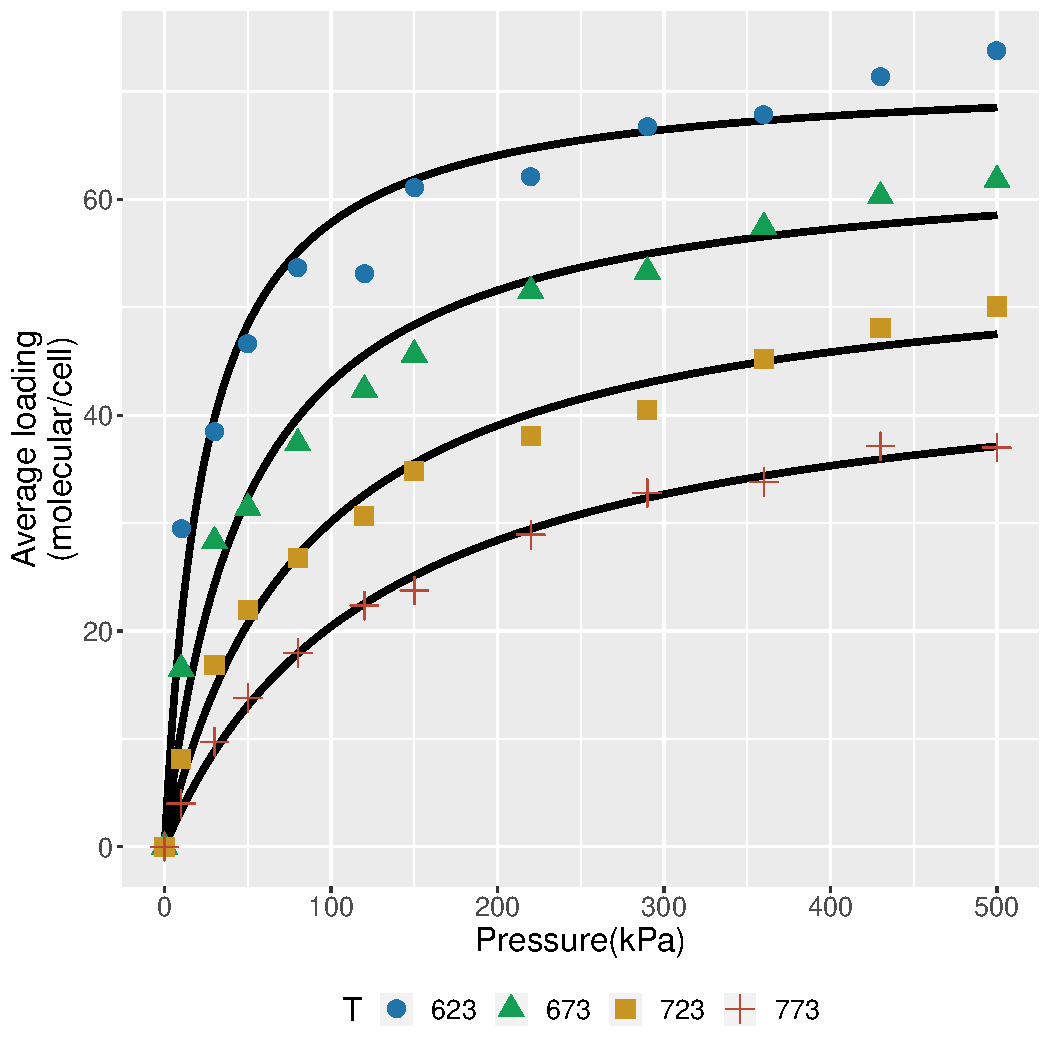
\includegraphics[width=2.7in]{figure/Adsorption/MacroPore20A.pdf}
    %\caption{fig2}
    \end{minipage}%
    }%
    \subfigure[丁酸甲酯在60Å介孔]{
    \begin{minipage}[t]{0.5\linewidth}
    \centering
    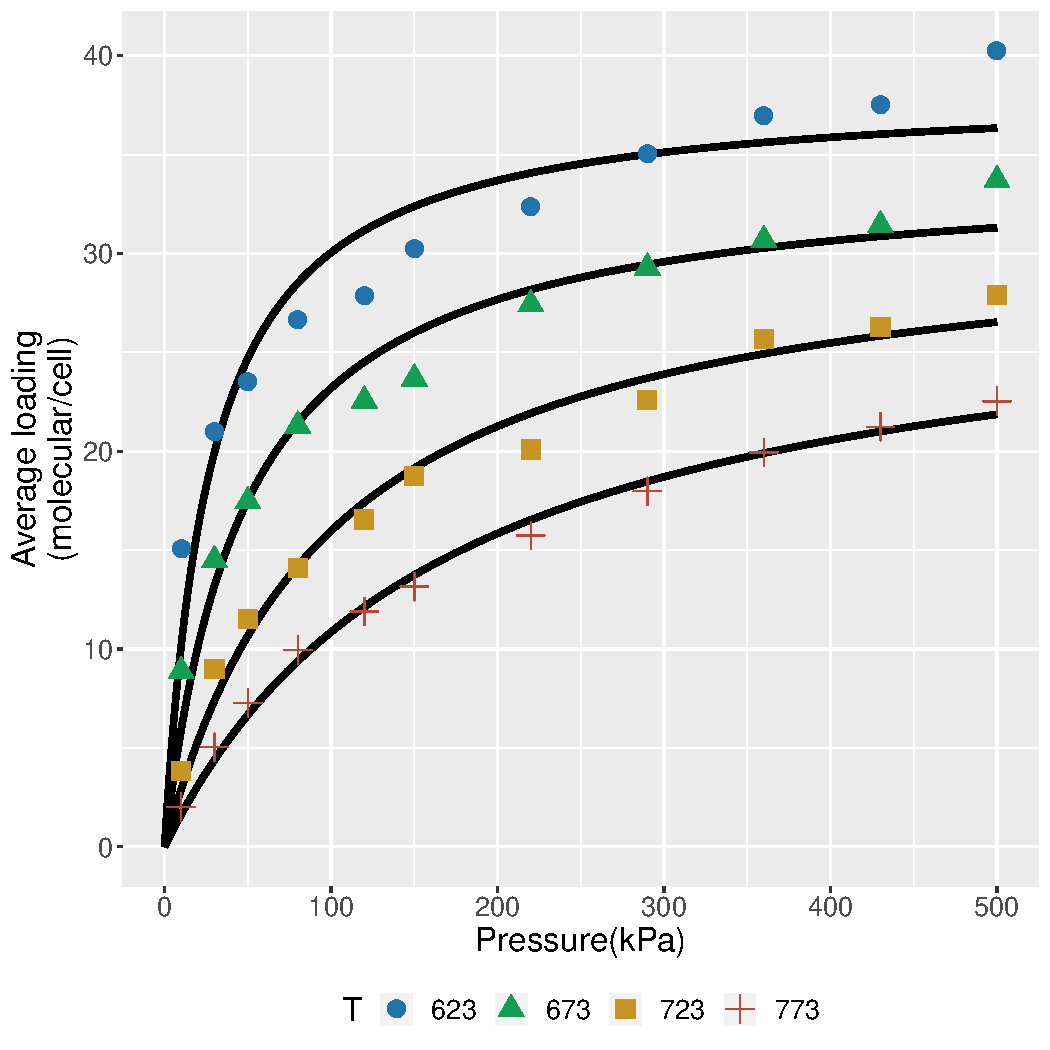
\includegraphics[width=2.7in]{figure/Adsorption/MacroPore60Anew.pdf}
    %\caption{fig2}
    \end{minipage}%
    }%
    \caption{丁酸甲酯和丁烯酸甲酯在微介孔H-ZSM-5分子筛的吸附等温线图}
    \label{fig:sA}
\end{figure}


\par{从\reffig{fig:sA}中可以看出:丁酸甲酯和丁烯酸甲酯的吸附等温线属于\uppercase\expandafter{\romannumeral1}型,满足朗格缪尔吸附方程,说明均为单层吸附,且吸附分子与分子筛之间的作用力占主导地位。对数据采用 \ref{郎格缪尔吸附} 所介绍的Langmuir公式进行拟合,公式如下:}
\begin{equation}
    V_{\mathrm{m}}=V_{\mathrm{m}^{\mathrm{a}}} \frac{b P}{1+b P}
\end{equation}
\par{式中:$V_{\mathrm{m}}$为平衡吸附量,$V_{\mathrm{m}^{a}}$ 为饱和吸附量,b为吸附平衡常数,P为压力。}
\par{拟合结果见\reftab{tab:sA}。}

\begin{table}[H]
	\small
	\centering
	\caption{在微介孔H-ZSM-5分子筛内丁酸甲酯和丁烯酸甲酯Langmuir公式拟合数据对比表}
	\begin{tabular}{p{2cm}<{\centering}p{2cm}<{\centering}p{1cm}<{\centering}p{4cm}<{\centering}p{2cm}<{\centering}p{2cm}<{\centering}}
        \toprule
        吸附质&孔径&\makecell*[c]{温度\\(K)}&\makecell*[c]{饱和吸附量\\(吸附分子数/超胞)}&\makecell*[c]{饱和吸附量\\(mmol/g)}&b\\
        \midrule
        \multirow{12}{*}{丁酸甲酯}&\multirow{4}{*}{微孔}&623&77.78&1.1238&0.1448\\
        &&673&71.83&1.0378&0.0559\\
        &&723&65.51&0.9465&0.0258\\
        &&773&60.22&0.8701&0.0115\\
        \cline{2-6}
        &\multirow{4}{*}{20Å介孔}&623&71.84&1.3502&0.0413\\
        &&673&64.31&1.2087&0.0203\\
        &&723&55.52&1.0435&0.0119\\
        &&773&46.66&0.8769&0.0078\\
        \cline{2-6}
        &\multirow{4}{*}{60Å介孔}&623&38.35&1.2271&0.0362\\
        &&673&34.31&1.0978&0.0209\\
        &&723&31.79&1.0172&0.0101\\
        &&773&29.28&0.9368&0.0059\\
        \hline
        \multirow{4}{*}{丁烯酸甲酯}&\multirow{4}{*}{微孔}&623&82.97&1.1987&0.2050\\
        &&673&79.44&1.1477&0.0642\\
        &&723&74.02&1.0694&0.0245\\
        &&773&64.77&0.9358&0.0132\\
		\bottomrule
	\end{tabular}
	\label{tab:sA}
\end{table}

\par{因为60Å介孔采用4×4×3的超胞进行模拟,所以为了和2×2×3超胞的微孔和20Å介孔在相同体积的条件下进行比较,60Å介孔的吸附量要除以四。}
\par{从\reftab{tab:sA}中可知,随着孔径的增大,丁酸甲酯的饱和吸附量越来越小。这是因为分子筛随着孔径的增大,相同体积下的活性吸附位(B位酸)数量减小(吸附位密度减小),以及微孔孔道(一般吸附位)数量减小,导致总的吸附位数量减小,从而丁酸甲酯的吸附量减小。而随着孔径的增大,单位质量下的分子筛吸附的丁酸甲酯分子的数量先增大,后减小,20Å介孔的吸附量最大,说明单位质量的20Å介孔的吸附效率最高,并不是孔径越大越好。在相同孔径的条件下,随着温度的增高,饱和吸附量减小,这是因为吸附是放热过程,低温有利于吸附。Langmuir公式中的b(吸附平衡常数)随着温度增大而减小,这是因为吸附平衡常数等于吸附速率常数比上解吸速率常数,随着温度的增高,吸附速率常数没有解吸速率常数增加得快。而在相同温度下,随着分子筛孔径的增大,丁酸甲酯的b(吸附平衡常数)减小,说明微孔与吸附分子之间的作用力更强,能更快的达到吸附饱和。}
\par{从\reftab{tab:sA}还可以看出,在623K$\sim$773K范围内,丁烯酸甲酯的饱和吸附量和b(吸附平衡常数)比丁酸甲酯的大,这是因为双键的存在,使丁烯酸甲酯具有更大的极性,而H-ZSM-5分子筛也是极性的,当吸附分子靠近吸附剂时,二者的电子结构发生变化而产生偶极矩,相互之间的主要作用力变成了更强的定向力和诱导力,从而吸附了更多的丁烯酸甲酯。}
\par{本文还研究了0$\sim$500kPa下乙酸甲酯到戊酸甲酯的吸附,随着吸附分子碳链长度的增加,脂肪酸甲酯在H-ZSM-5分子筛上的吸附也具有一定的规律。\reffig{fig:C2_C5}展示了不同碳链长度的脂肪酸甲酯在H-ZSM-5分子筛的吸附等温线。}

\begin{figure}[H]
    \centering
        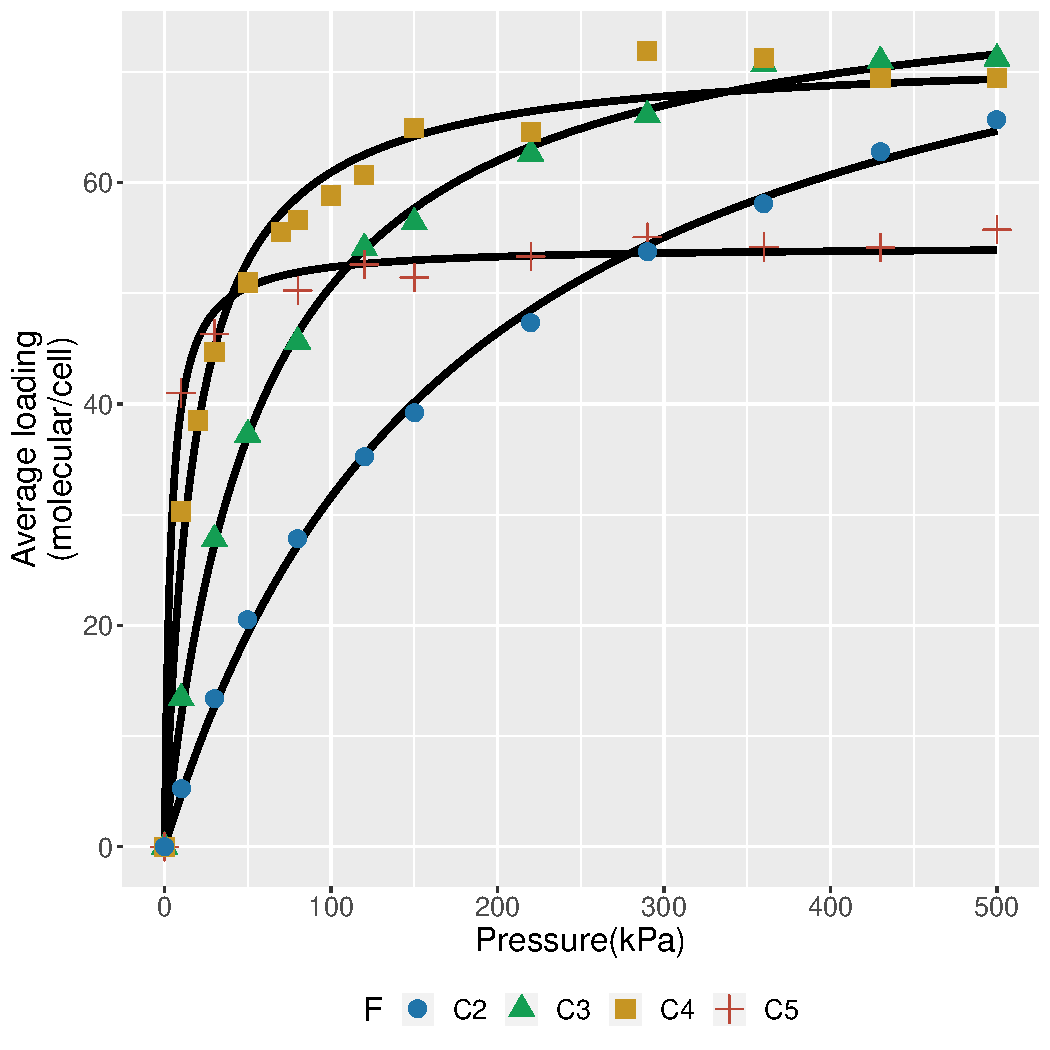
\includegraphics[width=0.5\linewidth]{figure/Adsorption/length.pdf}
    \caption{乙酸甲酯至戊酸甲酯在微孔H-ZSM-5分子筛内的吸附等温线图}
    \label{fig:C2_C5}
\end{figure}
\par{从\reffig{fig:C2_C5}可以看到,随着碳链长度的增加,脂肪酸甲酯在HZSM-5分子筛上的吸附量下降,b(吸附平衡常数)不断增大,通过 \ref{checking} 可知,油酸甲酯(十八烷酸甲酯)的b高达2.92。这是因为链长越大,分子筛对它的范德华力越大,就能越快地达到吸附平衡,但链长增大所引起的空间位阻的增大导致了其吸附量减小。具体拟合数据见\reftab{tab:C2_C5}。}
\begin{table}[H]
	\small
	\centering
	\caption{不同链长的脂肪酸甲酯Langmuir公式拟合数据对比表}
	\begin{tabular}{p{3cm}<{\centering}p{4cm}<{\centering}p{2.5cm}<{\centering}p{2.5cm}<{\centering}}
        \toprule
        分子&\makecell*[c]{饱和吸附量\\(吸附分子数/超胞)}&\makecell*[c]{饱和吸附量\\(mmol/g)}&b\\
        \midrule
        乙酸甲酯&87.59&1.2655&0.0056\\
        丙酸甲酯&79.84&1.1535&0.0173\\
        丁酸甲酯&71.83&1.0378&0.0559\\
        戊酸甲酯&54.29&0.7844&0.2703\\
		\bottomrule
	\end{tabular}
	\label{tab:C2_C5}
\end{table}
\subsubsection{等量吸附热}
\par{等量吸附热是固体吸附气体过程中衡量吸附质分子吸附性能的一个重要参数,被定义为吸附质分子在由游离的气体分子状态转为被吸附剂分子吸附时的状态所放出的热量。}
\par{在巨正则蒙特卡洛法(GCMC)的模拟中,等量吸附热Q是依据下式计算得出:}
\begin{equation}
    Q=R T-\frac{\left\langle N U_{N}\right\rangle-\langle N\rangle\left\langle U_{N}\right\rangle}{\left\langle N^{2}\right\rangle\langle N\rangle^{2}}
    \end{equation}
\par{式中:$N$为吸附分子数;$R$为体系开式温度;$R$为理想气体常数;$U_N$为吸附相势能;$ \langle \rangle$为系综平均。}

\par{\reffig{fig:sH1}为丁酸甲酯分子在673K,微介孔H-ZSM-5分子筛中的等量吸附热随吸附量和压力的变化图。}
\begin{figure}[H]
    \centering

    \subfigure[等量吸附热随压力变化图]{
        \begin{minipage}[t]{0.5\linewidth}
        \centering
        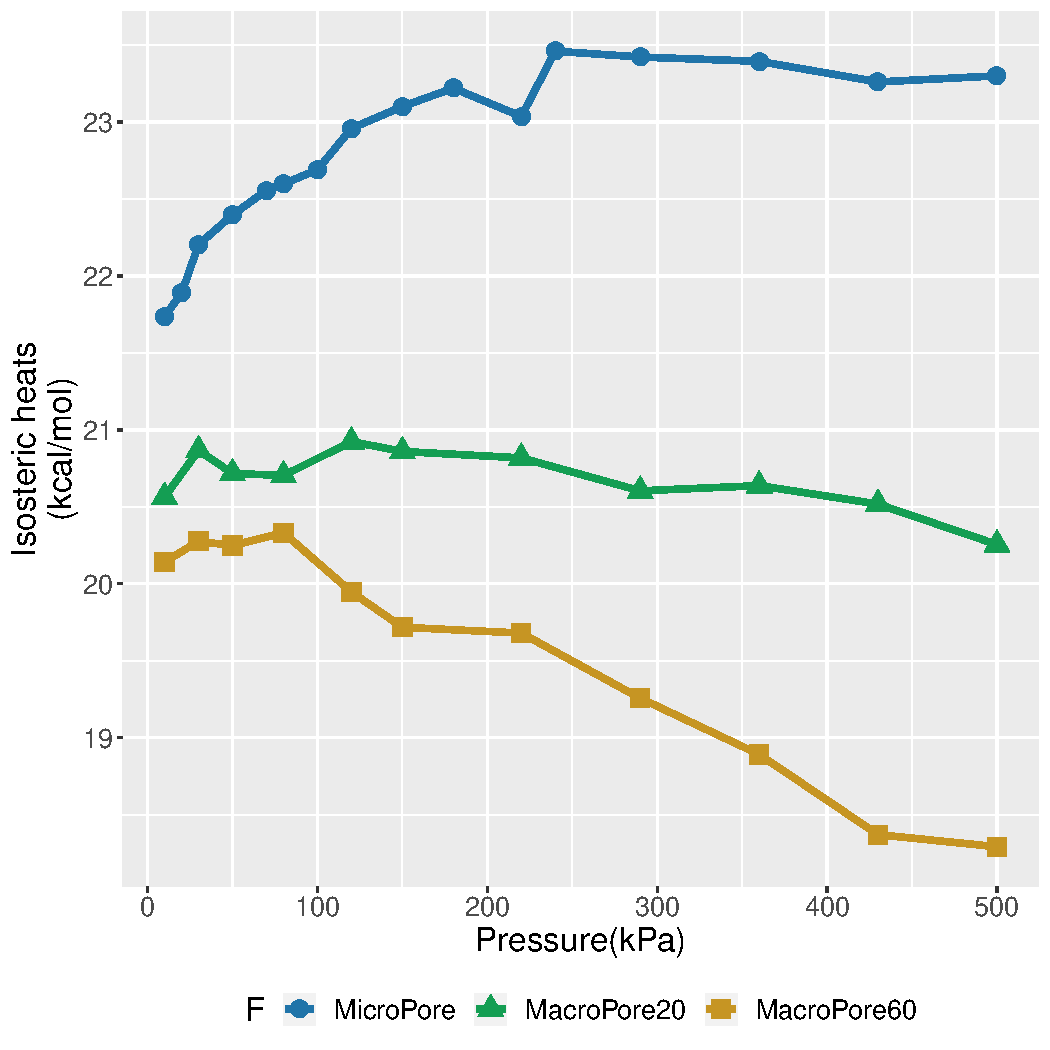
\includegraphics[width=2.8in]{figure/Adsorption/Heat673.pdf}
        %\caption{fig1}
        \end{minipage}%
    }%
    \subfigure[等量吸附热随吸附量变化图]{
        \begin{minipage}[t]{0.5\linewidth}
        \centering
        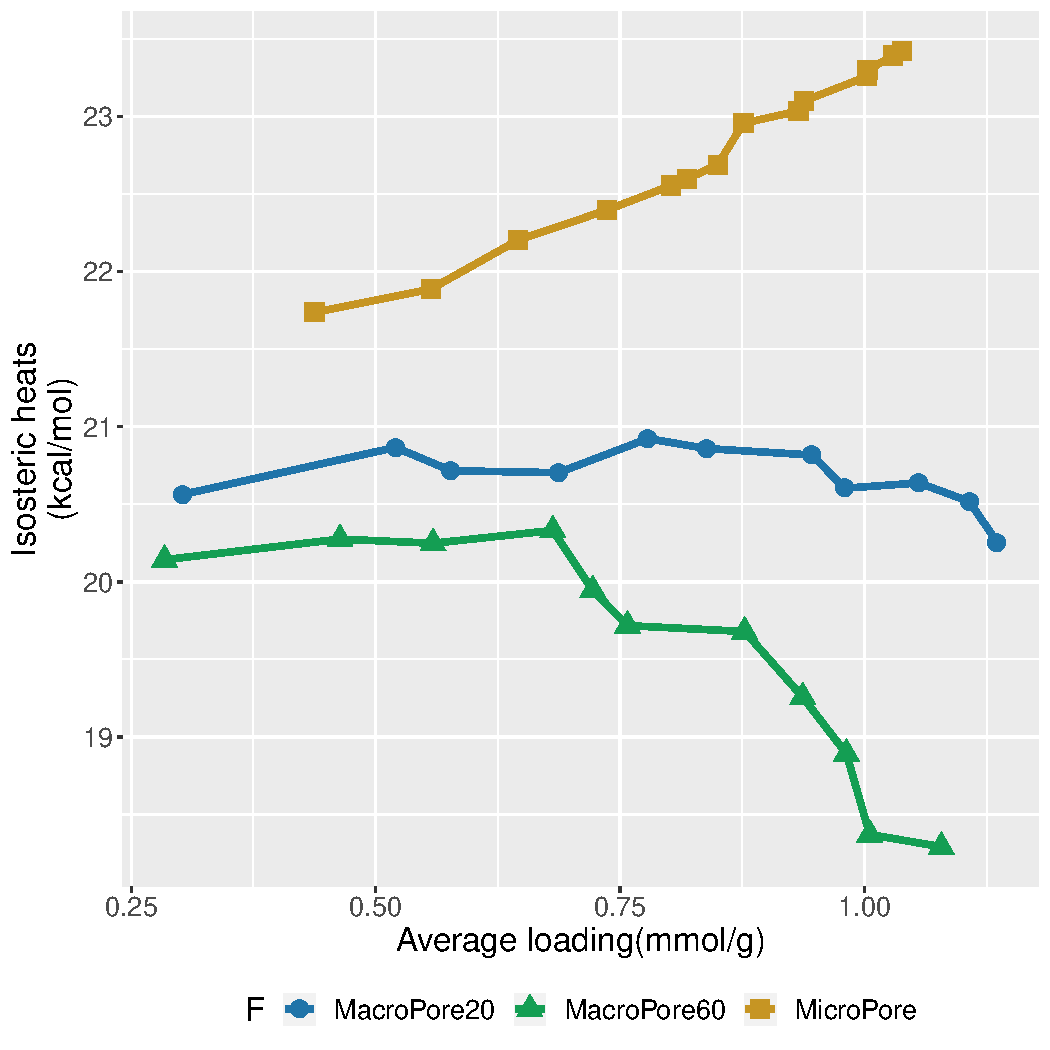
\includegraphics[width=2.8in]{figure/Adsorption/111.pdf}
        %\caption{fig1}
        \end{minipage}%
    }%
    \caption{丁酸甲酯在673K下不同孔径分子筛中的等量吸附热随吸附量和压力的变化图}
    \label{fig:sH1}
\end{figure}
\par{从\reffig{fig:sH1}中可以看出,在相同压力或者吸附量的条件下,60Å介孔 < 20Å介孔<微孔的等量吸附热,说明孔径越大,等量吸附热越小。翟冬\cite{翟冬2011C4}认为吸附热主要受两部分作用力影响:吸附质与吸附剂之间的相互作用力以及吸附剂分子之间的相互作用力。因为从 \ref{吸附等温线} 可知,吸附分子与微孔之间的作用力大于与介孔的(在微孔中的吸附平衡常数比在介孔的大),所以微孔的更加稳定,放出的热就更多。}
\par{在微孔分子筛中,随着压力的增大,等量吸附热逐渐增大,直到达到最大值,随着吸附量的增大,等量吸附热线性增大。因为当吸附量增加时,吸附质分子之间距离的变小,吸附质分子之间的相互作用将越来越大,单位数量的吸附质之间的作用力引起的吸附热将越来越大,但吸附分子与吸附剂之间的相互作用并不会随吸附量的增大而增大,所以丁酸甲酯在微孔内的吸附热的变化本质上是由于吸附质分子之间的相互作用增大而引起的。}
\par{而介孔的等量吸附热随着压力或者吸附量的增大,等量吸附热先增大后减小,有一个最大值。这是因为在分子筛中引入介孔为吸附分子提供了较短的扩散路径和较高的扩散速率\cite{liu2012adsorption}。在低压下丁酸甲酯在介孔分子筛孔道吸附固定的效率较高,优先占据活性吸附位(B位酸),放出较高吸附热量\cite{2017介孔材料吸附气相多环芳烃实验及分子模拟研究},再加上上文所说的吸附量增加,吸附分子之间作用力增大,等量吸附热增大,所以刚开始等量吸附热会随吸附量(压力)增大而增大;而随着压力升高,吸附量增加量减小,逐渐达到饱和,吸附分子之间距离减小所增加的吸附热的影响减小,活性位点(B位酸)也逐渐被占据完,吸附质分子转向一般的吸附位点(孔道),放出的吸附热下降,吸附量增加所导致的吸附热增加量小于减少量,于是等量吸附热随着吸附量增加而下降。}
\par{而60Å介孔的等量吸附热最高点时的压力小于20Å介孔的是因为在60Å介孔分子筛中,到活性位点的路径更加短,而且在相同体积的条件下,60Å介孔的活性吸附位(B位酸)的个数原小于20Å介孔的个数,所以压力更低(吸附量更少)的条件下,即可完成所有活性吸附位点的吸附。}


\par{\reffig{fig:sH2}展示了温度对等量吸附热的影响,从图中可以看出温度越高,吸附热越小,并且在相同吸附量下,介孔中的吸附热比微孔的对温度更加敏感。因为吸附热是当气体分子固定在吸附位时,吸附分子因速度变慢导致动能减小,从而释放热量,而温度升高,吸附分子运动变剧烈,所以转化的动能(吸附热)变少,而介孔分子筛中的吸附位在介孔周围,附着在吸附位上的吸附分子受到的空间位阻相对较小,所以随着温度的增大,运动幅度相较微孔增加得更大,动能增加量更大,于是释放的热量减少得更多。}

\begin{figure}[H]
    \centering

    \subfigure[微孔压力]{
    \begin{minipage}[t]{0.5\linewidth}
    \centering
    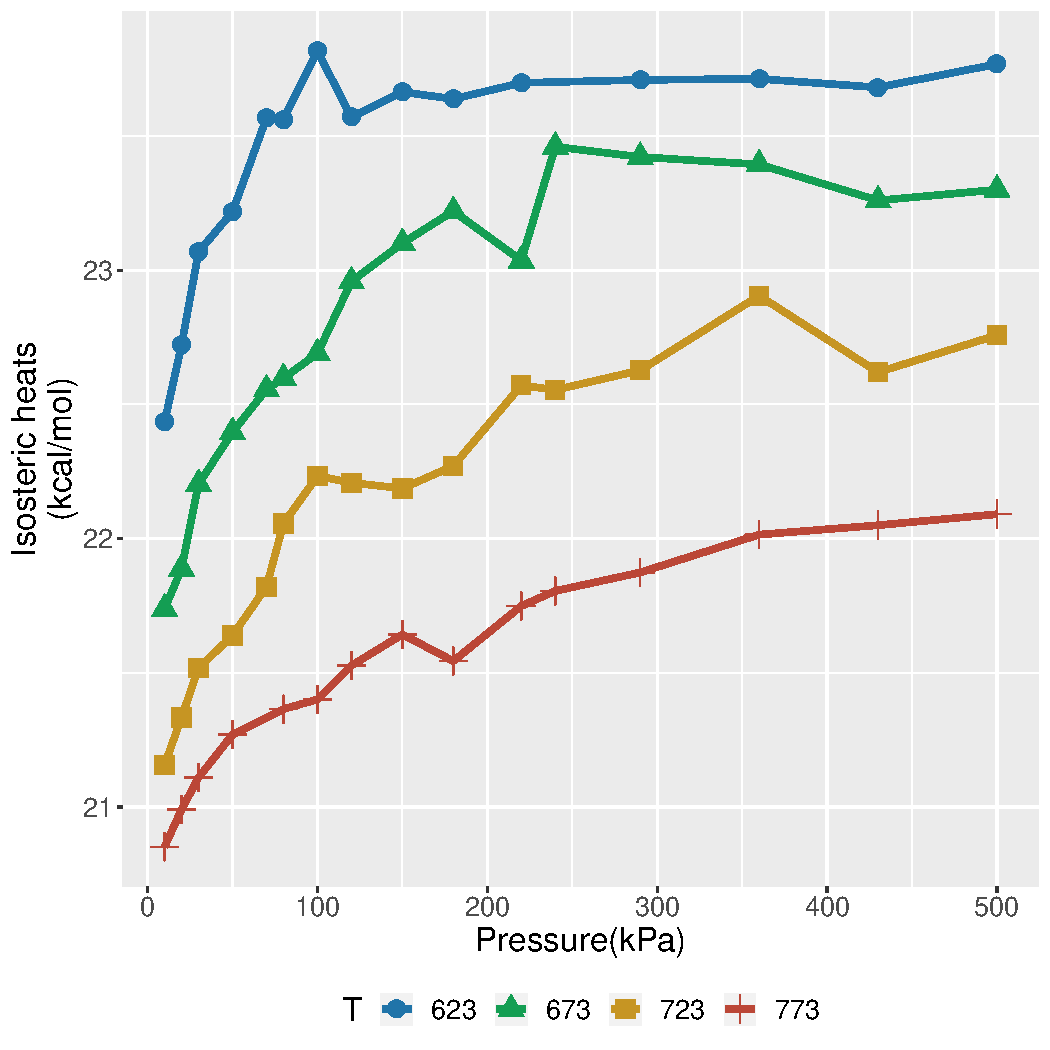
\includegraphics[width=2.7in]{figure/Adsorption/MicroPoreH.pdf}
    %\caption{fig1}
    \end{minipage}%
    }%
    \subfigure[微孔吸附量]{
    \begin{minipage}[t]{0.5\linewidth}
    \centering
    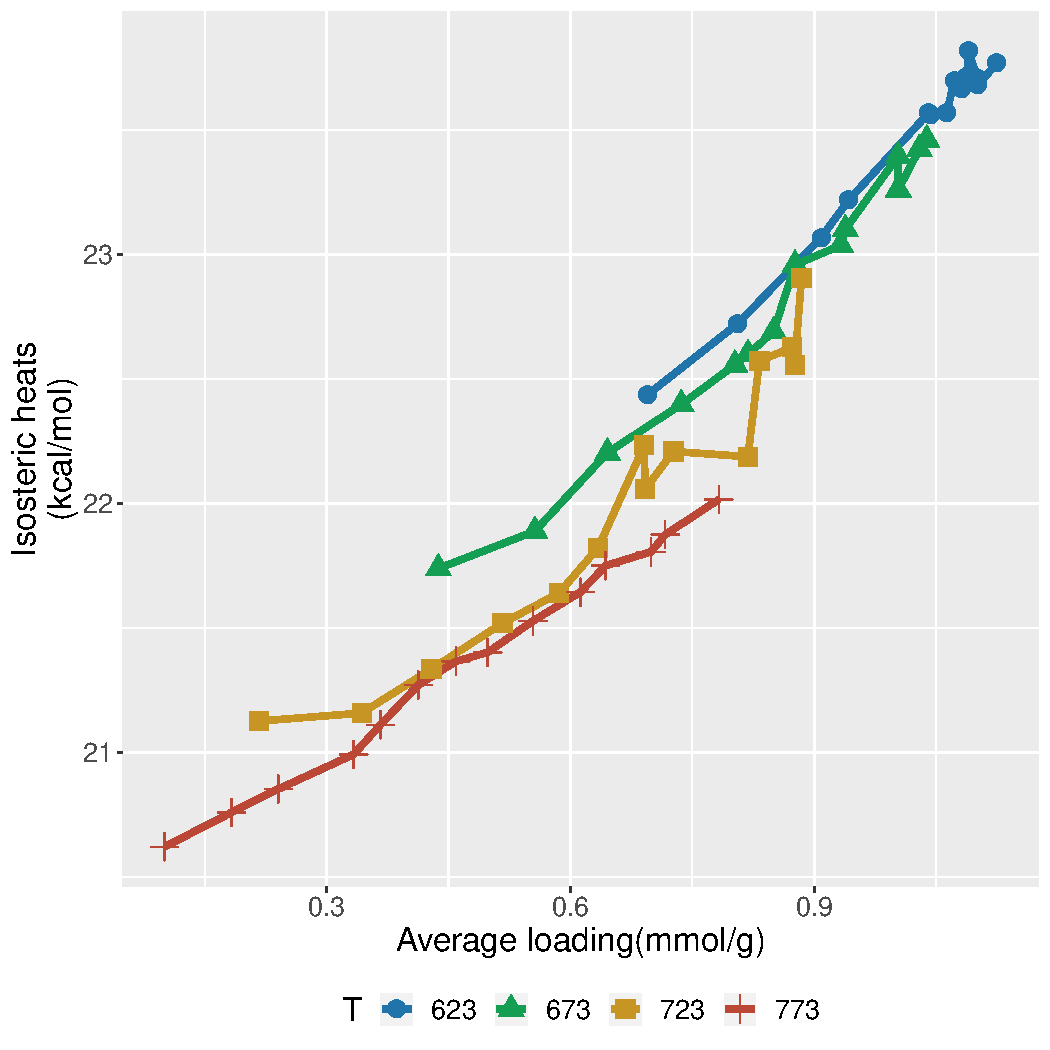
\includegraphics[width=2.7in]{figure/Adsorption/222MM.pdf}
    %\caption{fig2}
    \end{minipage}%
    }%

    \subfigure[20Å介孔压力]{
    \begin{minipage}[t]{0.5\linewidth}
    \centering
    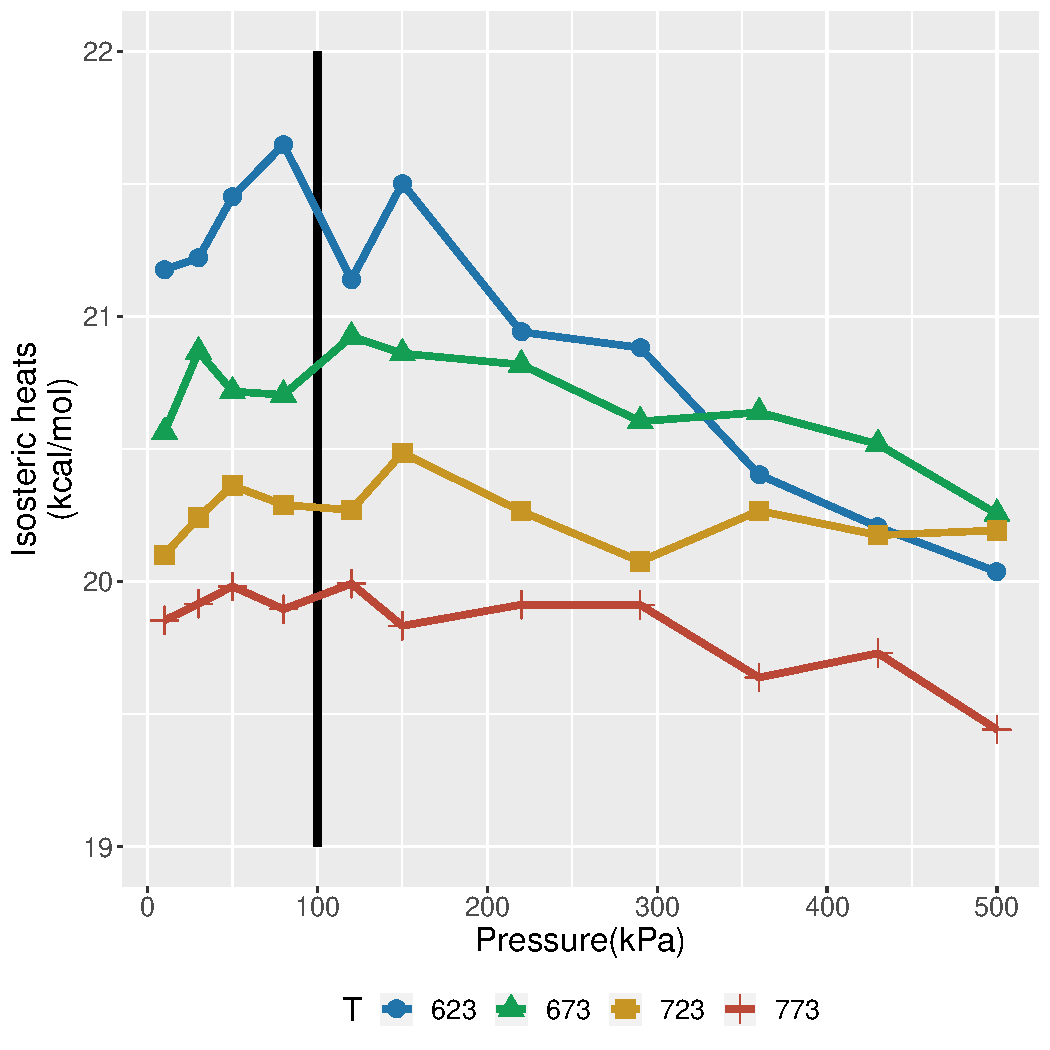
\includegraphics[width=2.7in]{figure/Adsorption/MacroPore20H.pdf}
    %\caption{fig2}
    \end{minipage}%
    }%
    \subfigure[20Å介孔吸附量]{
    \begin{minipage}[t]{0.5\linewidth}
    \centering
    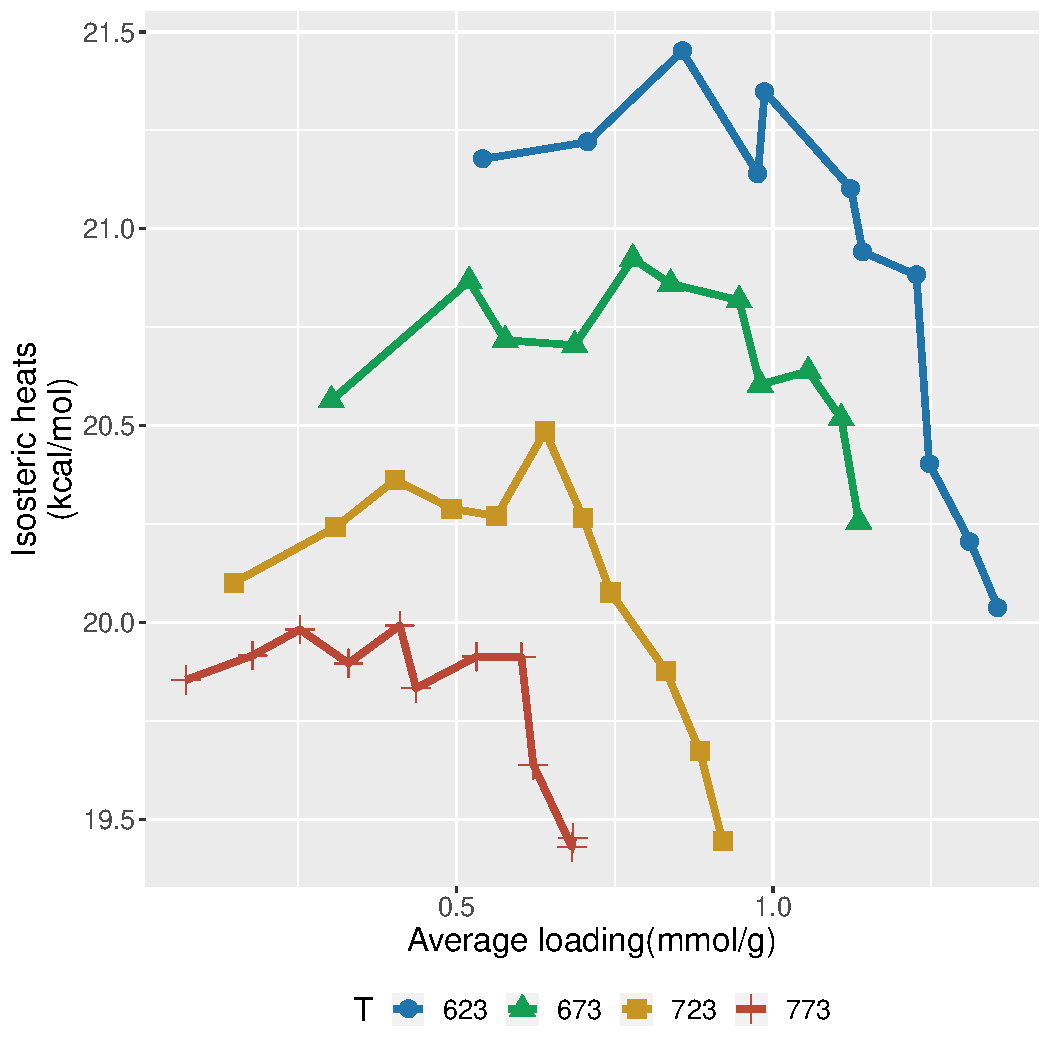
\includegraphics[width=2.7in]{figure/Adsorption/222M20.pdf}
    %\caption{fig2}
    \end{minipage}%
    }%

    \subfigure[60Å介孔压力]{
    \begin{minipage}[t]{0.5\linewidth}
    \centering
    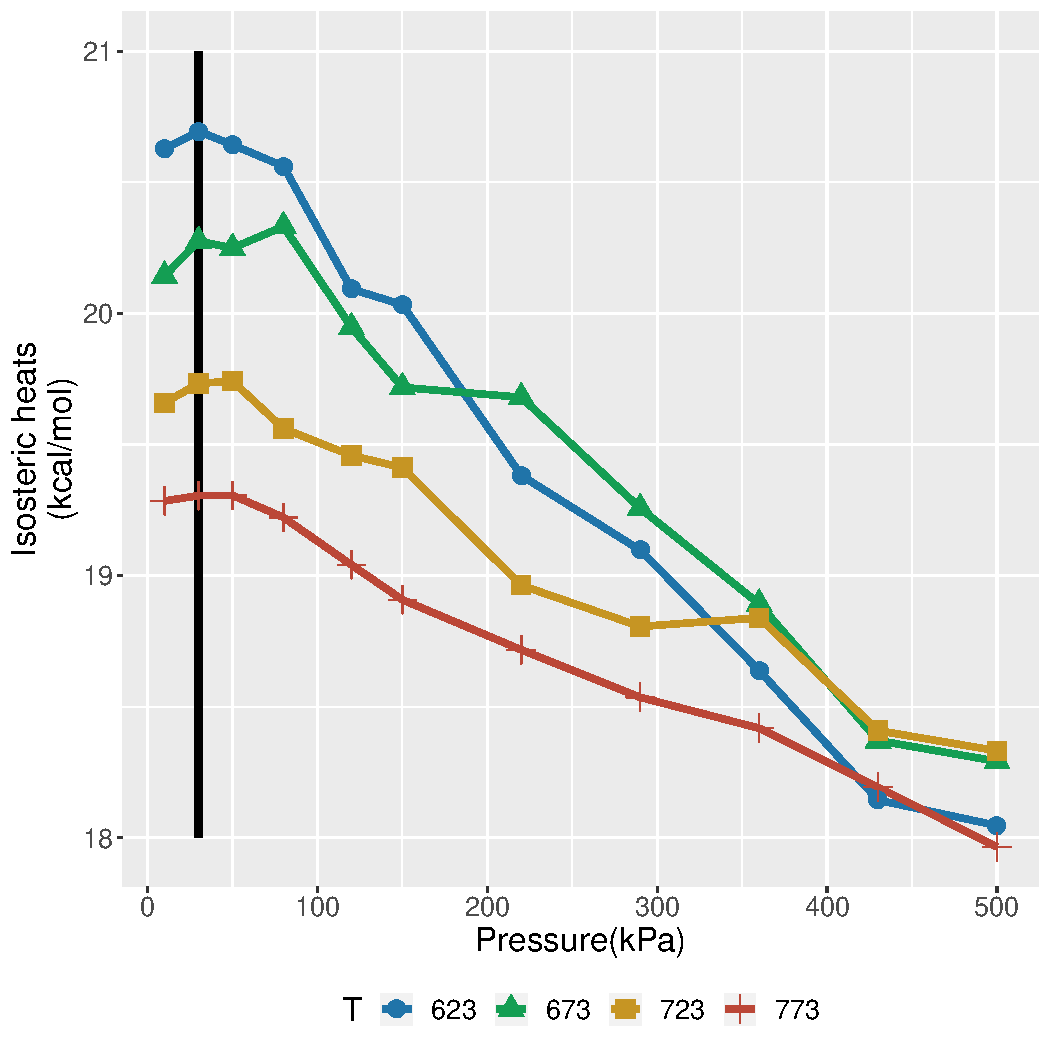
\includegraphics[width=2.7in]{figure/Adsorption/MacroPore60H.pdf}
    %\caption{fig2}
    \end{minipage}%
    }%
    \subfigure[60Å介孔吸附量]{
    \begin{minipage}[t]{0.5\linewidth}
    \centering
    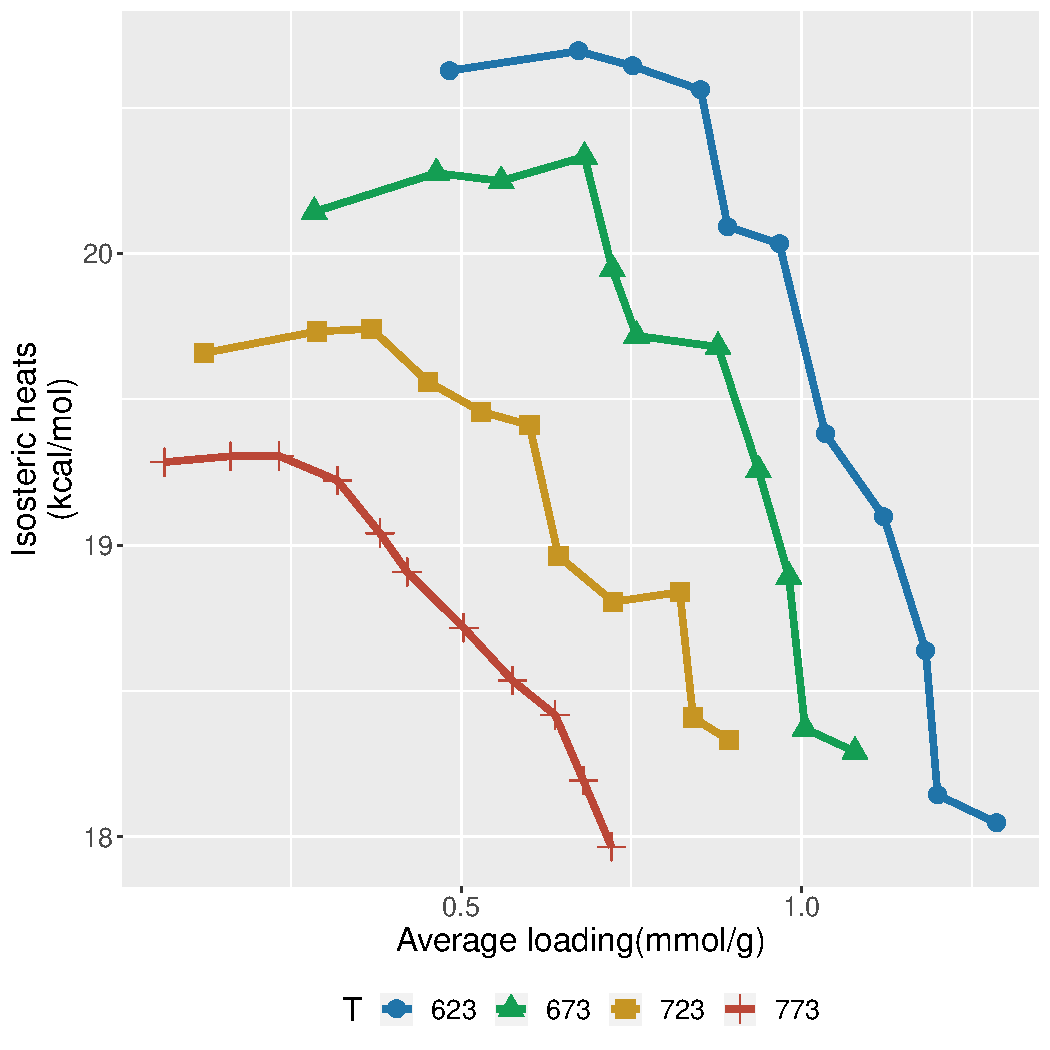
\includegraphics[width=2.7in]{figure/Adsorption/222M60.pdf}
    %\caption{fig2}
    \end{minipage}%
    }%
    \caption{丁酸甲酯在不同温度下的等量吸附热随压力和吸附量的变化图}
    \label{fig:sH2}
\end{figure}
\par{通过\reffig{fig:sH2}还发现在介孔中的等量吸附热最大值所对应的压力几乎不随温度发生变化,孔径越大,结果越明显。这是因为在60Å介孔的条件下,饱和吸附量从623K到773K下降了23.7\%,而20Å介孔下降了35.1\%,说明在相同压力下,在20Å介孔中的吸附量对温度更加敏感,而吸附量改变,等量吸附热则会改变,所以当温度改变时,在对温度相对不敏感的60Å介孔中的等量吸附热变化较小。}


% \par{本文计算了不同链长的脂肪酸甲酯在微孔H-ZSM-5上的等量吸附热随吸附量的变化曲线。如\reffig{fig:C2_C5H}所示,随着吸附量的增大,等量吸附热线性增大。这是因为随着吸附量的增大,吸附质分子之间的距离变短,从而吸附质分子之间的作用力变大,放出更多的热量,从而单位数量的吸附质分子之间的作用力引起的热量更大,而吸附质与吸附剂之间的作用力并不会随着吸附质分子数量的增大而增大,所以最后随着吸附量的增大,等量吸附热变大。}

% \begin{figure}[H]
%     \centering
%         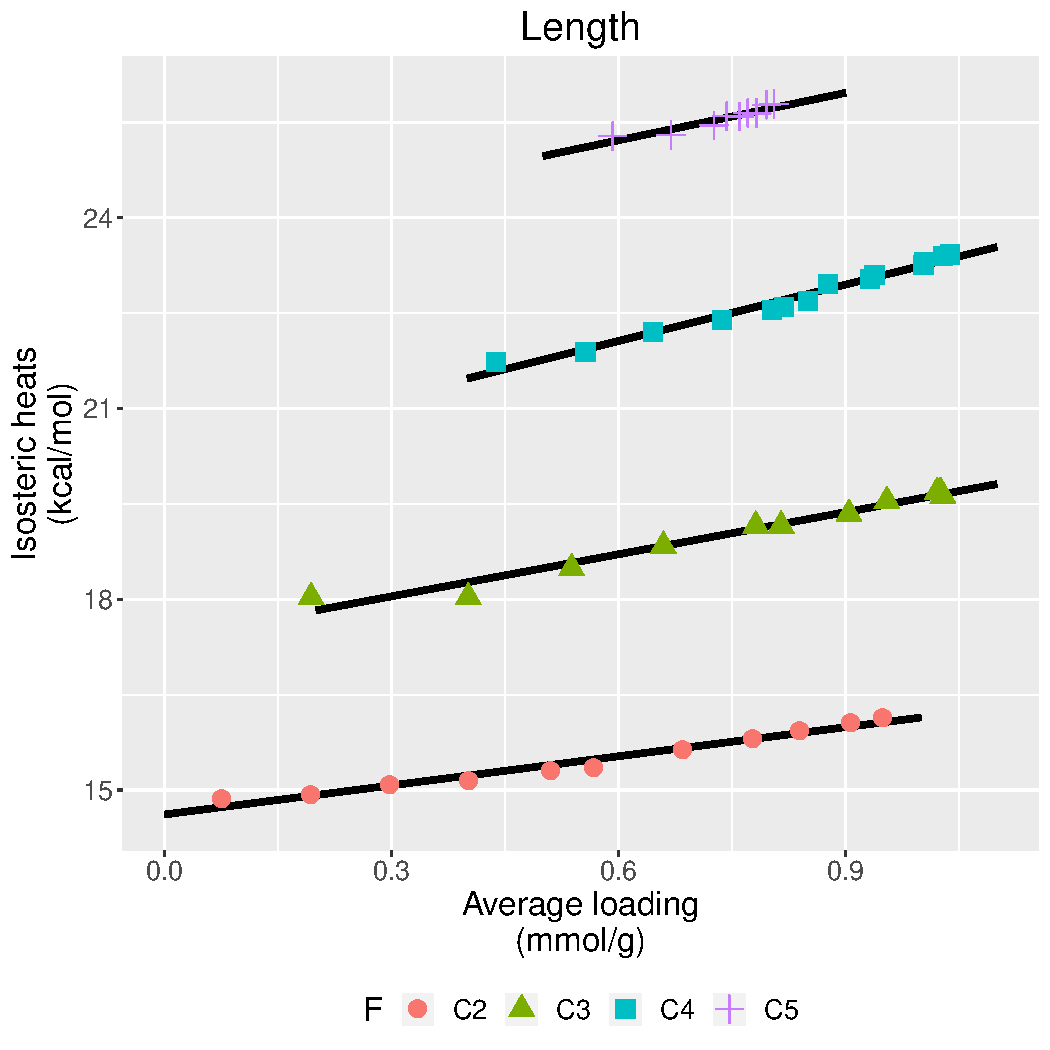
\includegraphics[width=0.6\linewidth]{figure/Adsorption/lengthheat.pdf}
%     \caption{乙酸甲酯至戊酸甲酯在微孔H-ZSM-5分子筛内的吸附热随吸附量的变化曲线图}
%     \label{fig:C2_C5H}
% \end{figure}
% \par{从\reffig{fig:C2_C5H}还发现,吸附热与链长呈直线关系,所以选取吸附量为0.6mmol/mg时的吸附热与链长作图,如所示\reffig{fig:C2_C5h}所示。R$^2$=0.9999,且每增加一个亚甲基,等量吸附热变增加3.24kcal/mol,约13.55kJ/mol。这个现象与实验报道的烷烃链长和吸附热呈线性关系,且每增加一个亚甲基等量吸附热就增加10kJ/mol\cite{yang1986use}的结果相似。}

% \begin{figure}[H]
%     \centering
%         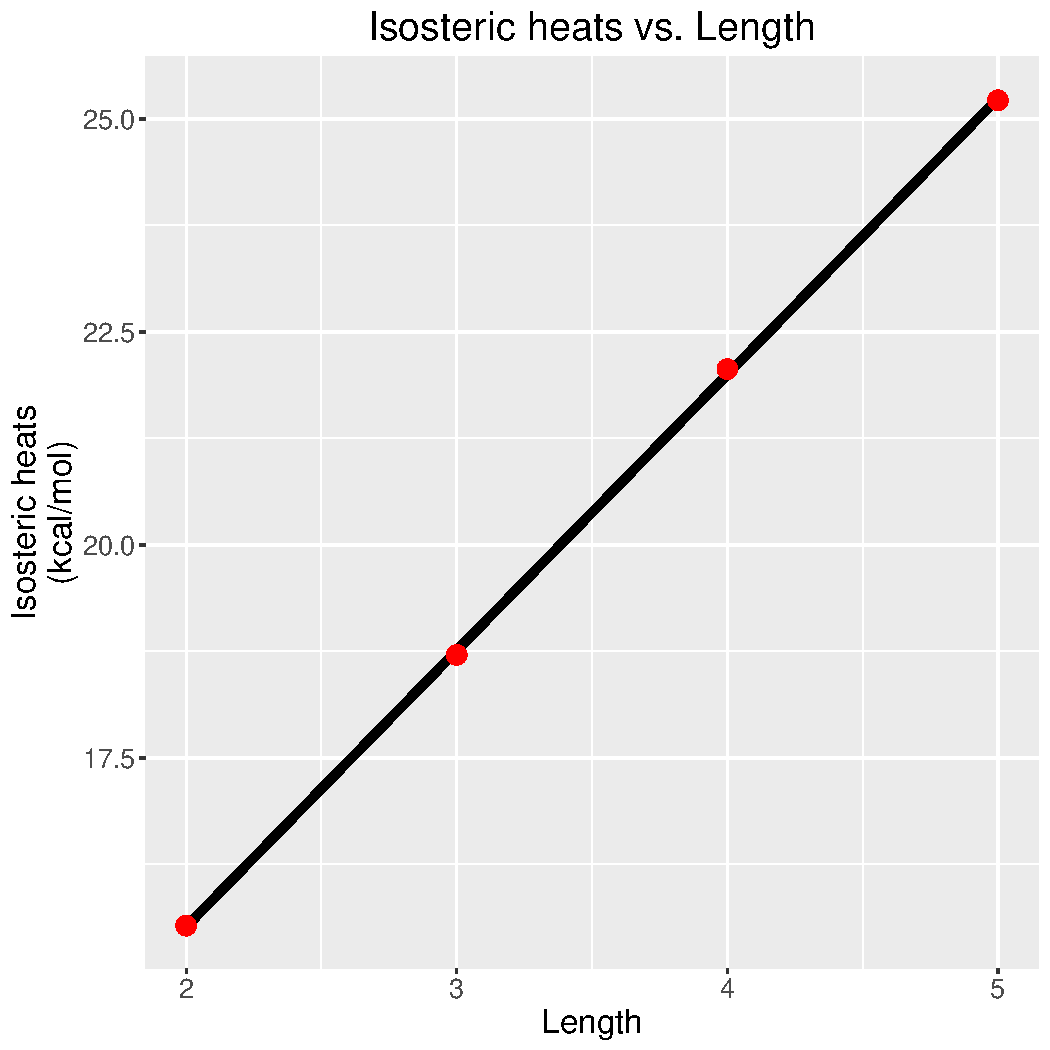
\includegraphics[width=0.6\linewidth]{figure/Adsorption/lengthH.pdf}
%     \caption{在微孔H-ZSM-5分子筛内的等量吸附热随吸附质链长的变化曲线}
%     \label{fig:C2_C5h}
% \end{figure}


\subsubsection{吸附位}
\par{本文研究了压力对吸附位置的影响,选取10kPa作为低压,1000kPa作为高压,温度取673K,结果如\ref{fig:loaction}所示。}


\begin{figure}[H]
    \centering

    \subfigure[低压A方向]{
    \begin{minipage}[t]{0.3333\linewidth}
    \centering
    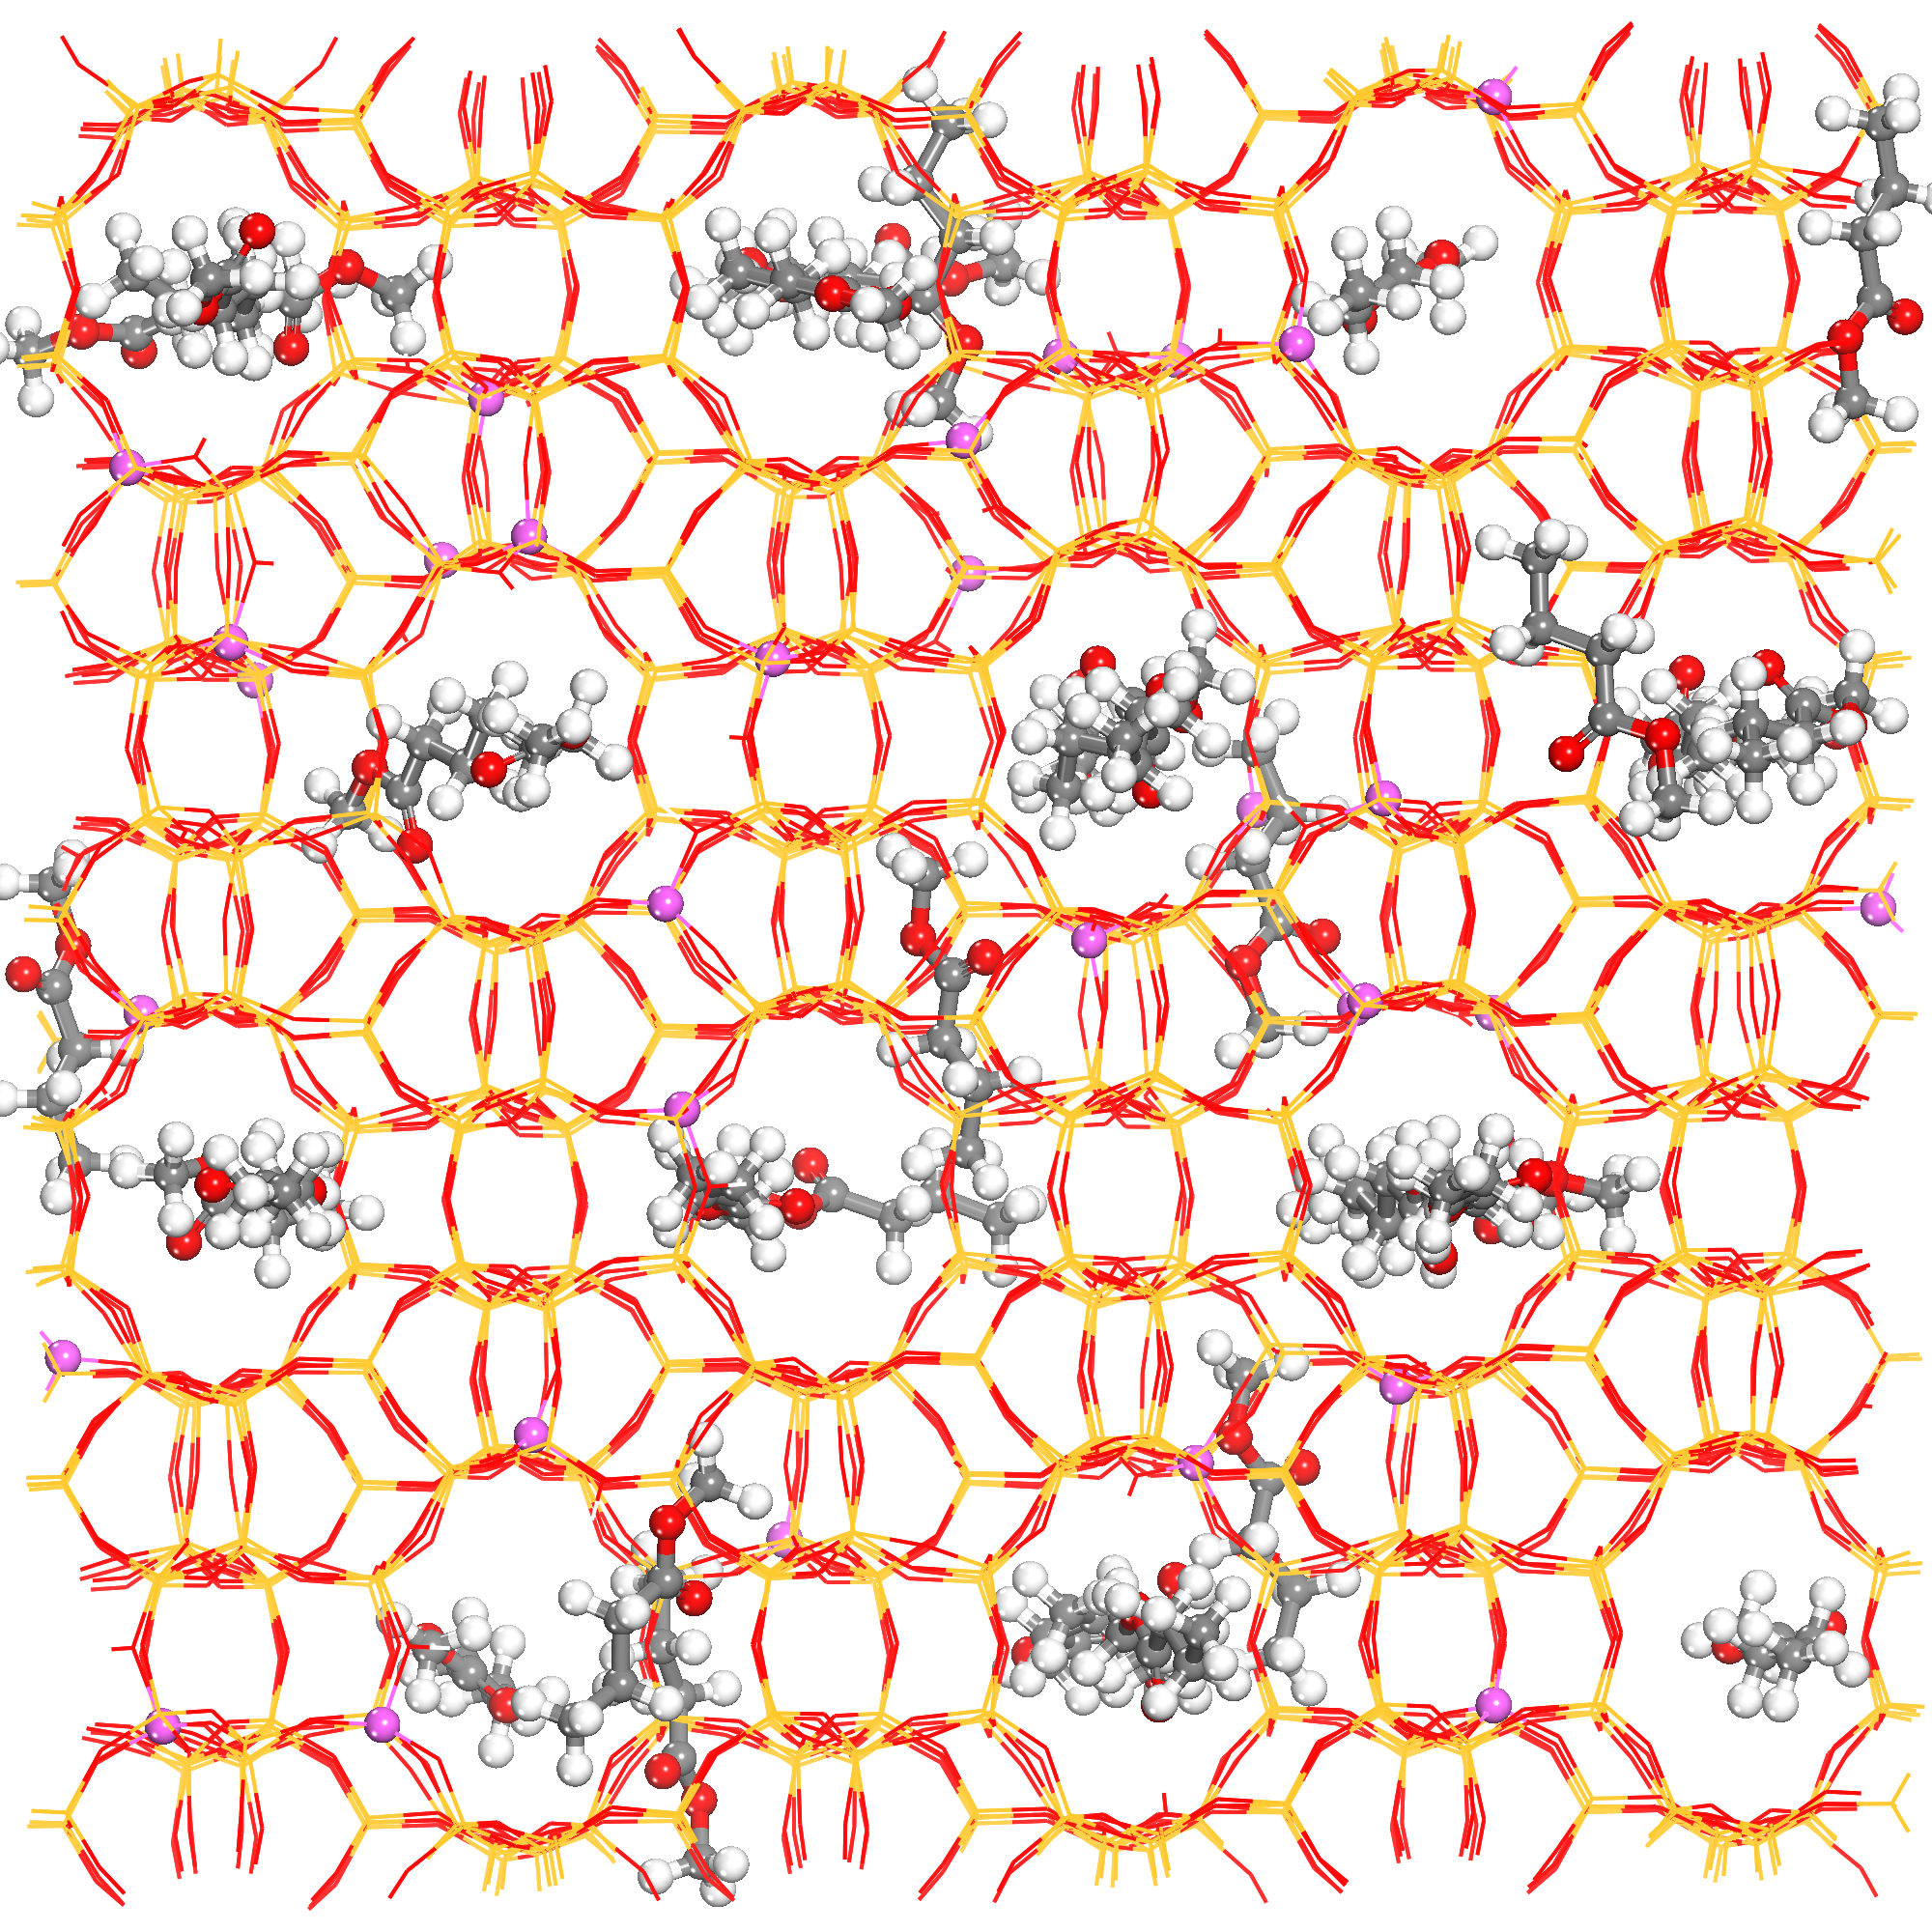
\includegraphics[width=1.8in]{figure/Adsorption/lowA.png}
    %\caption{fig1}
    \end{minipage}%
    }%
    \subfigure[低压B方向]{
    \begin{minipage}[t]{0.3333\linewidth}
    \centering
    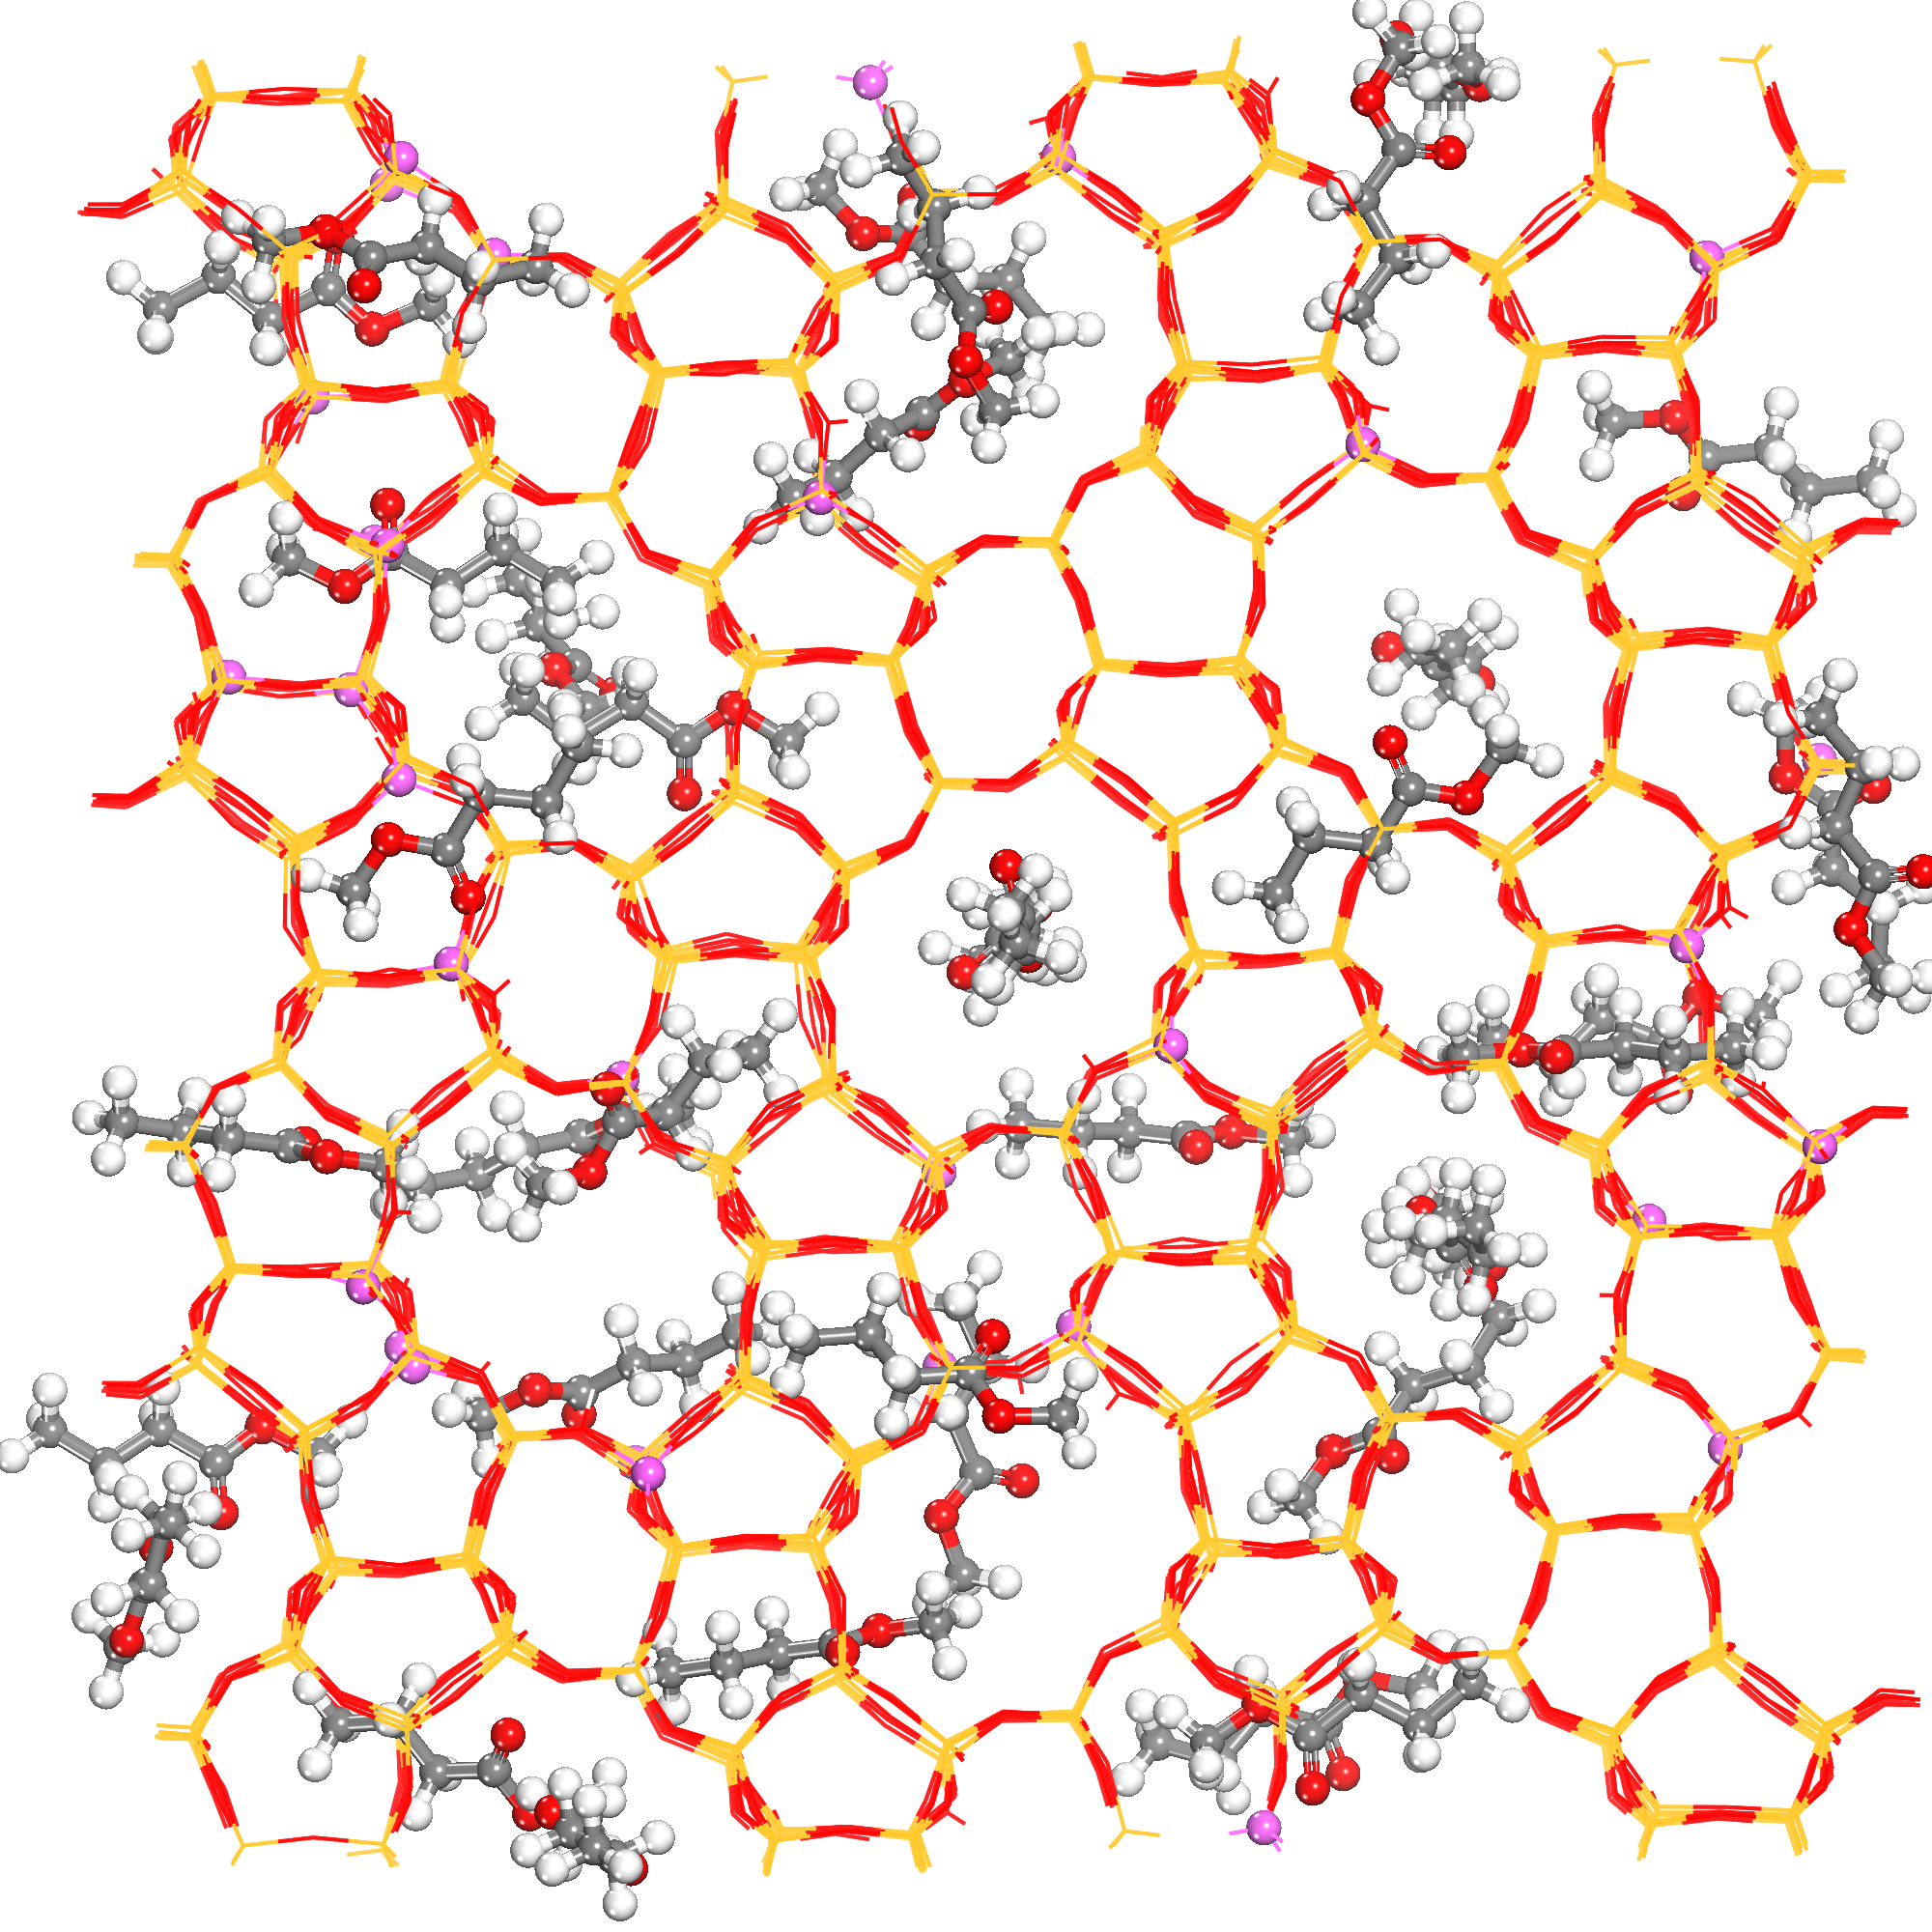
\includegraphics[width=1.8in]{figure/Adsorption/lowB.png}
    %\caption{fig2}
    \end{minipage}%
    }%
    \subfigure[低压C方向]{
    \begin{minipage}[t]{0.3333\linewidth}
    \centering
    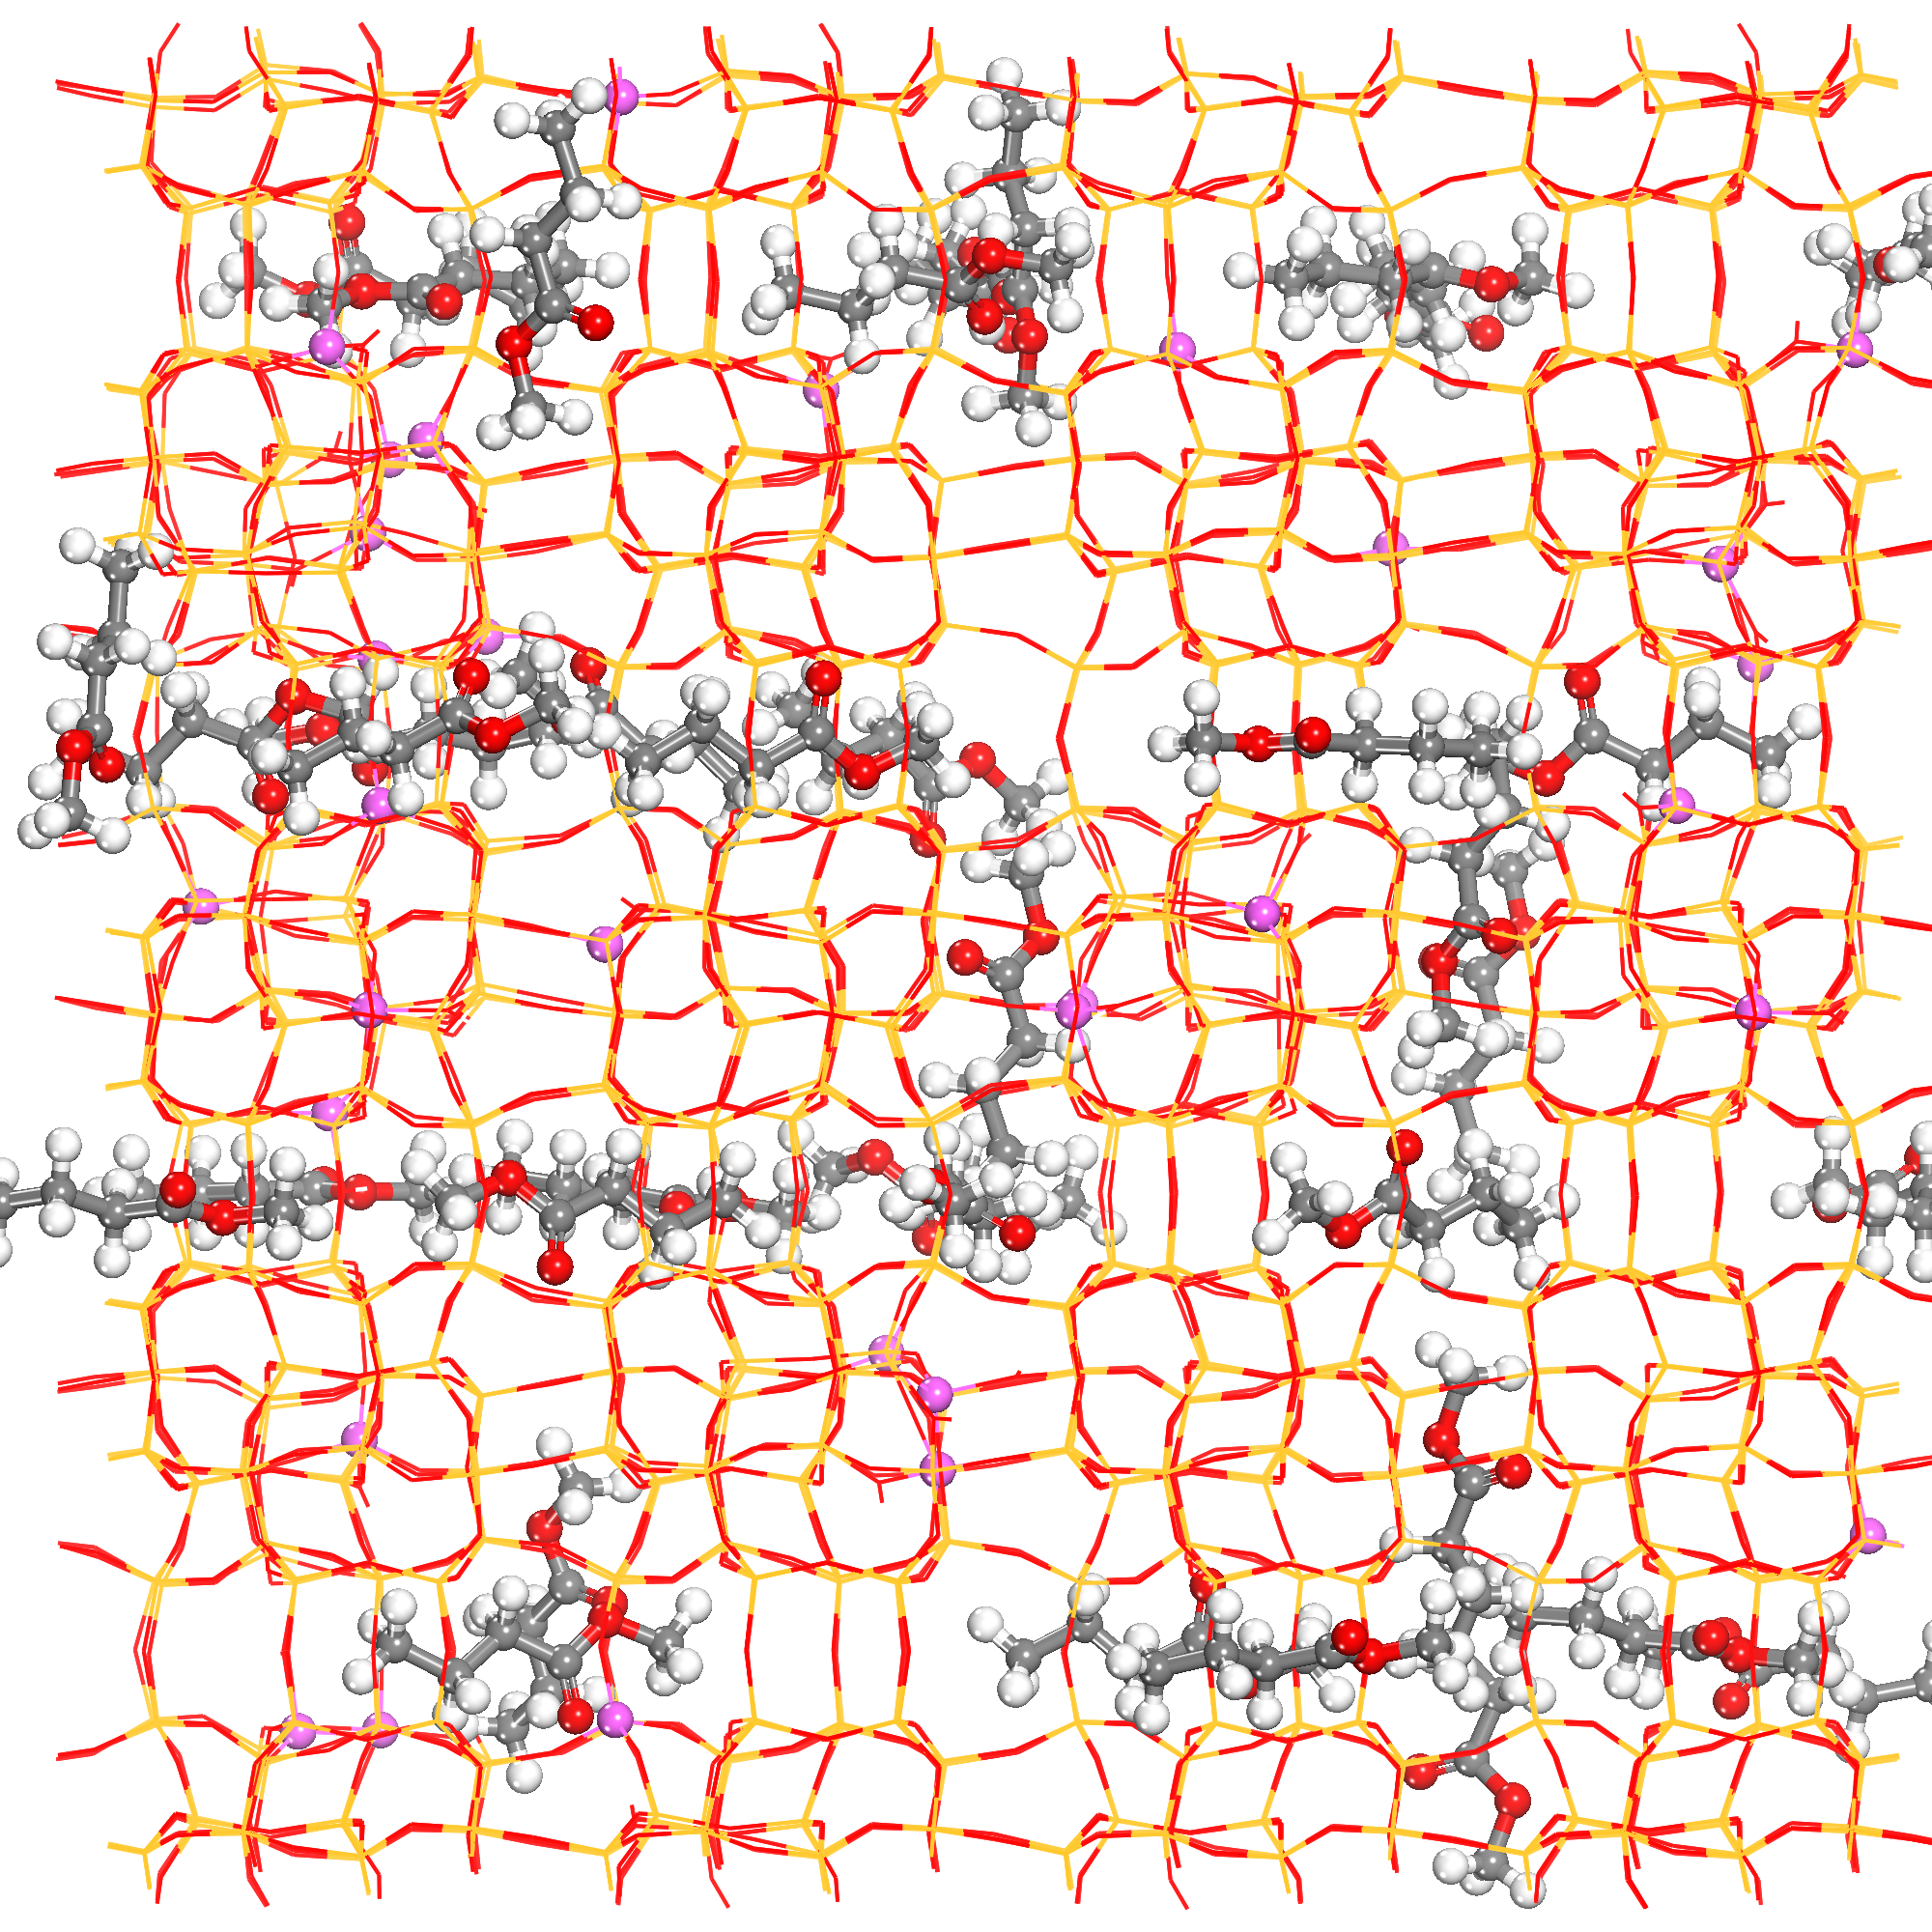
\includegraphics[width=1.8in]{figure/Adsorption/lowC.png}
    %\caption{fig2}
    \end{minipage}%
    }%

    \subfigure[高压A方向]{
    \begin{minipage}[t]{0.3333\linewidth}
    \centering
    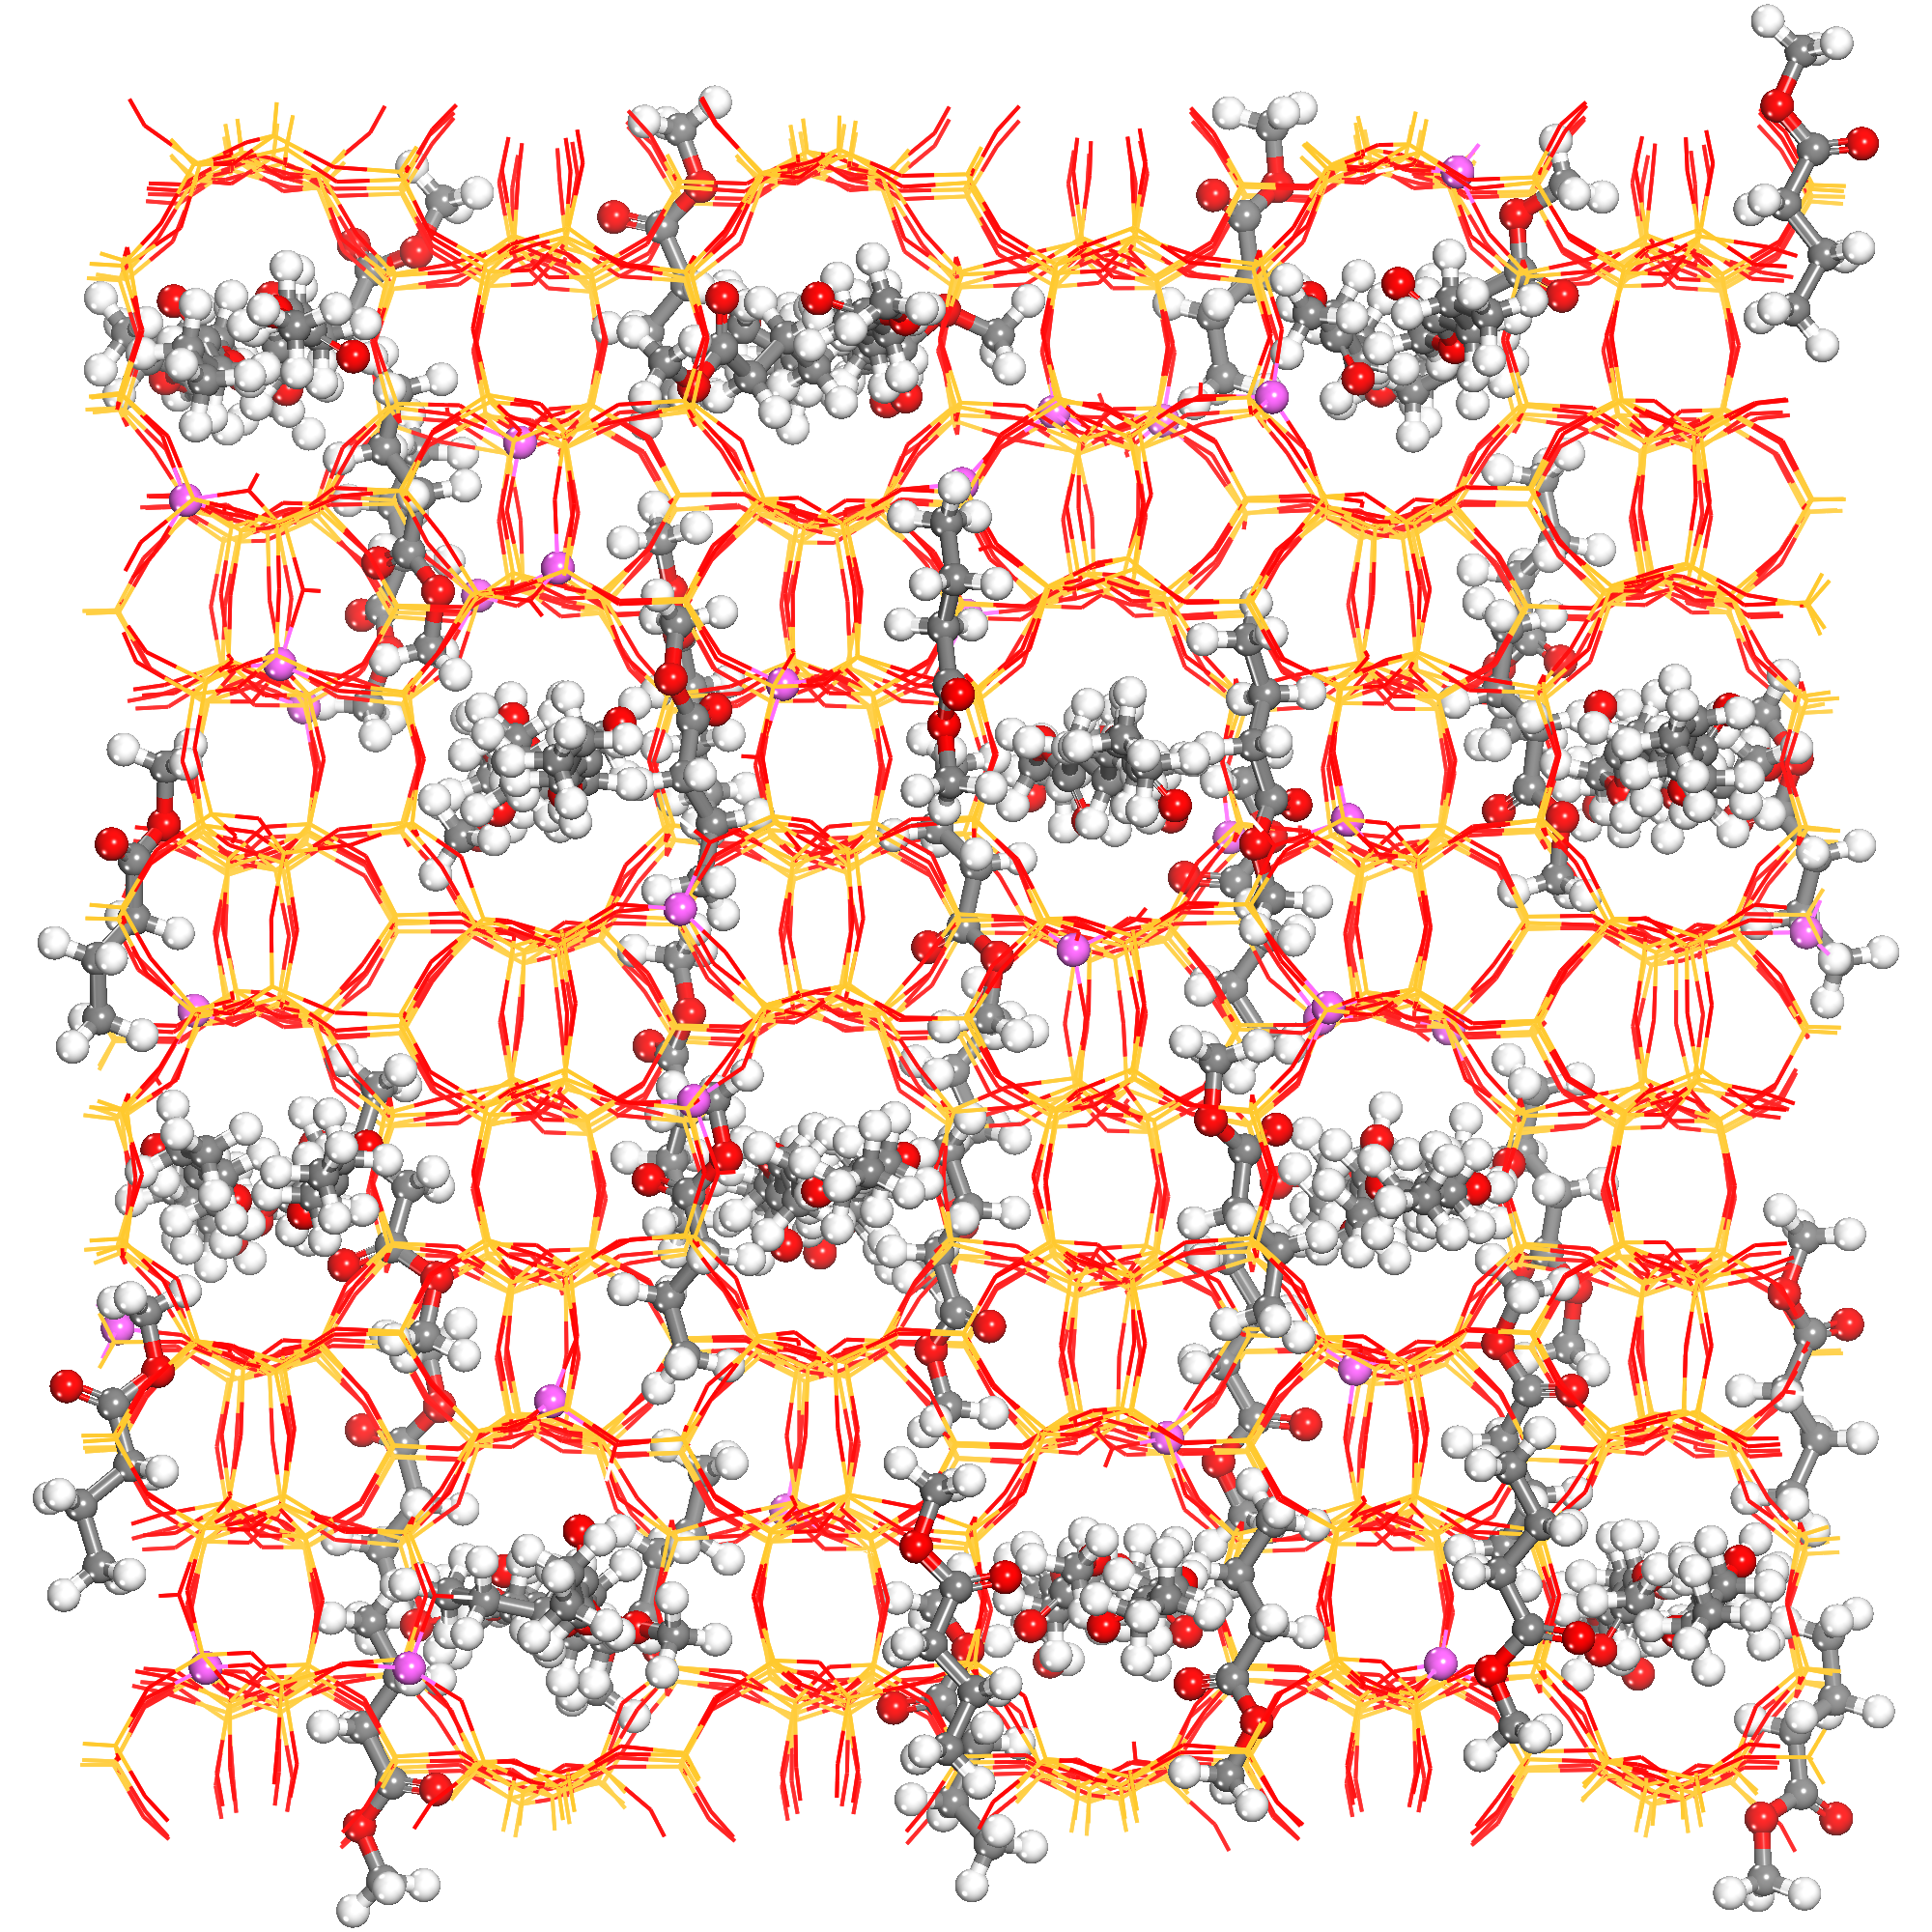
\includegraphics[width=1.8in]{figure/Adsorption/highA.png}
    %\caption{fig2}
    \end{minipage}%
    }%
    \subfigure[高压B方向]{
    \begin{minipage}[t]{0.3333\linewidth}
    \centering
    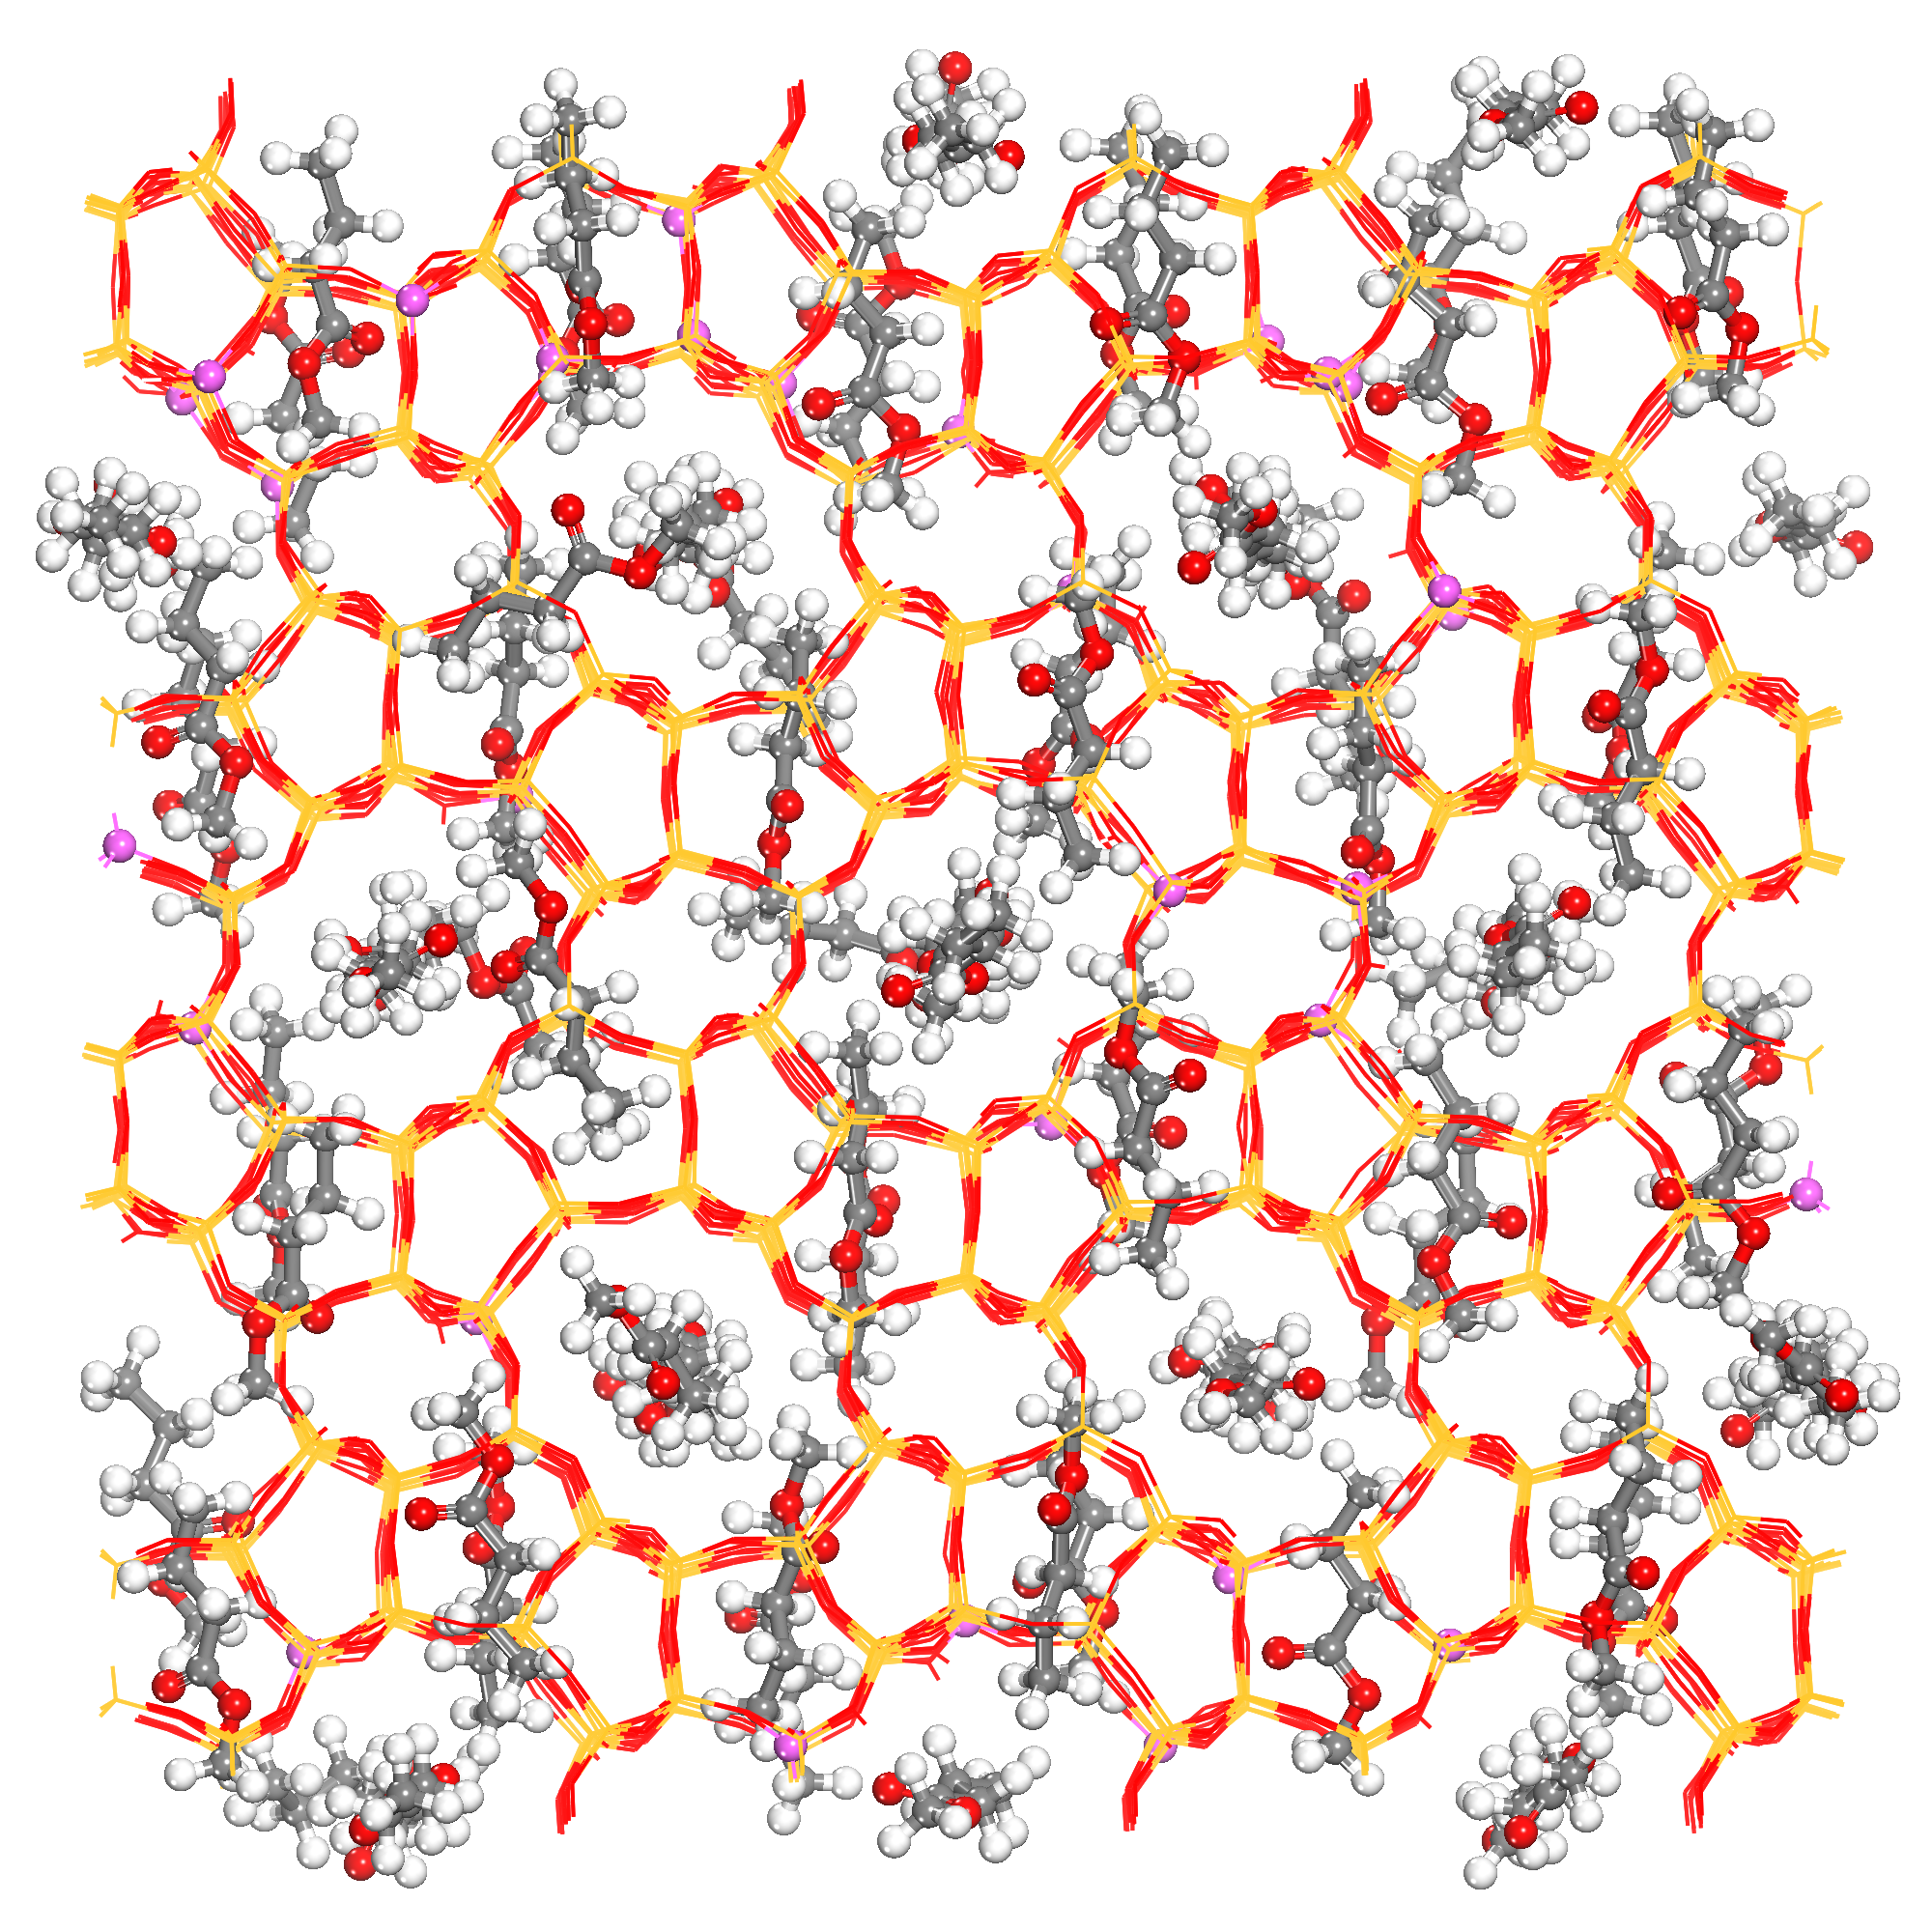
\includegraphics[width=1.8in]{figure/Adsorption/highB.png}
    %\caption{fig2}
    \end{minipage}%
    }%
    \subfigure[高压C方向]{
    \begin{minipage}[t]{0.3333\linewidth}
    \centering
    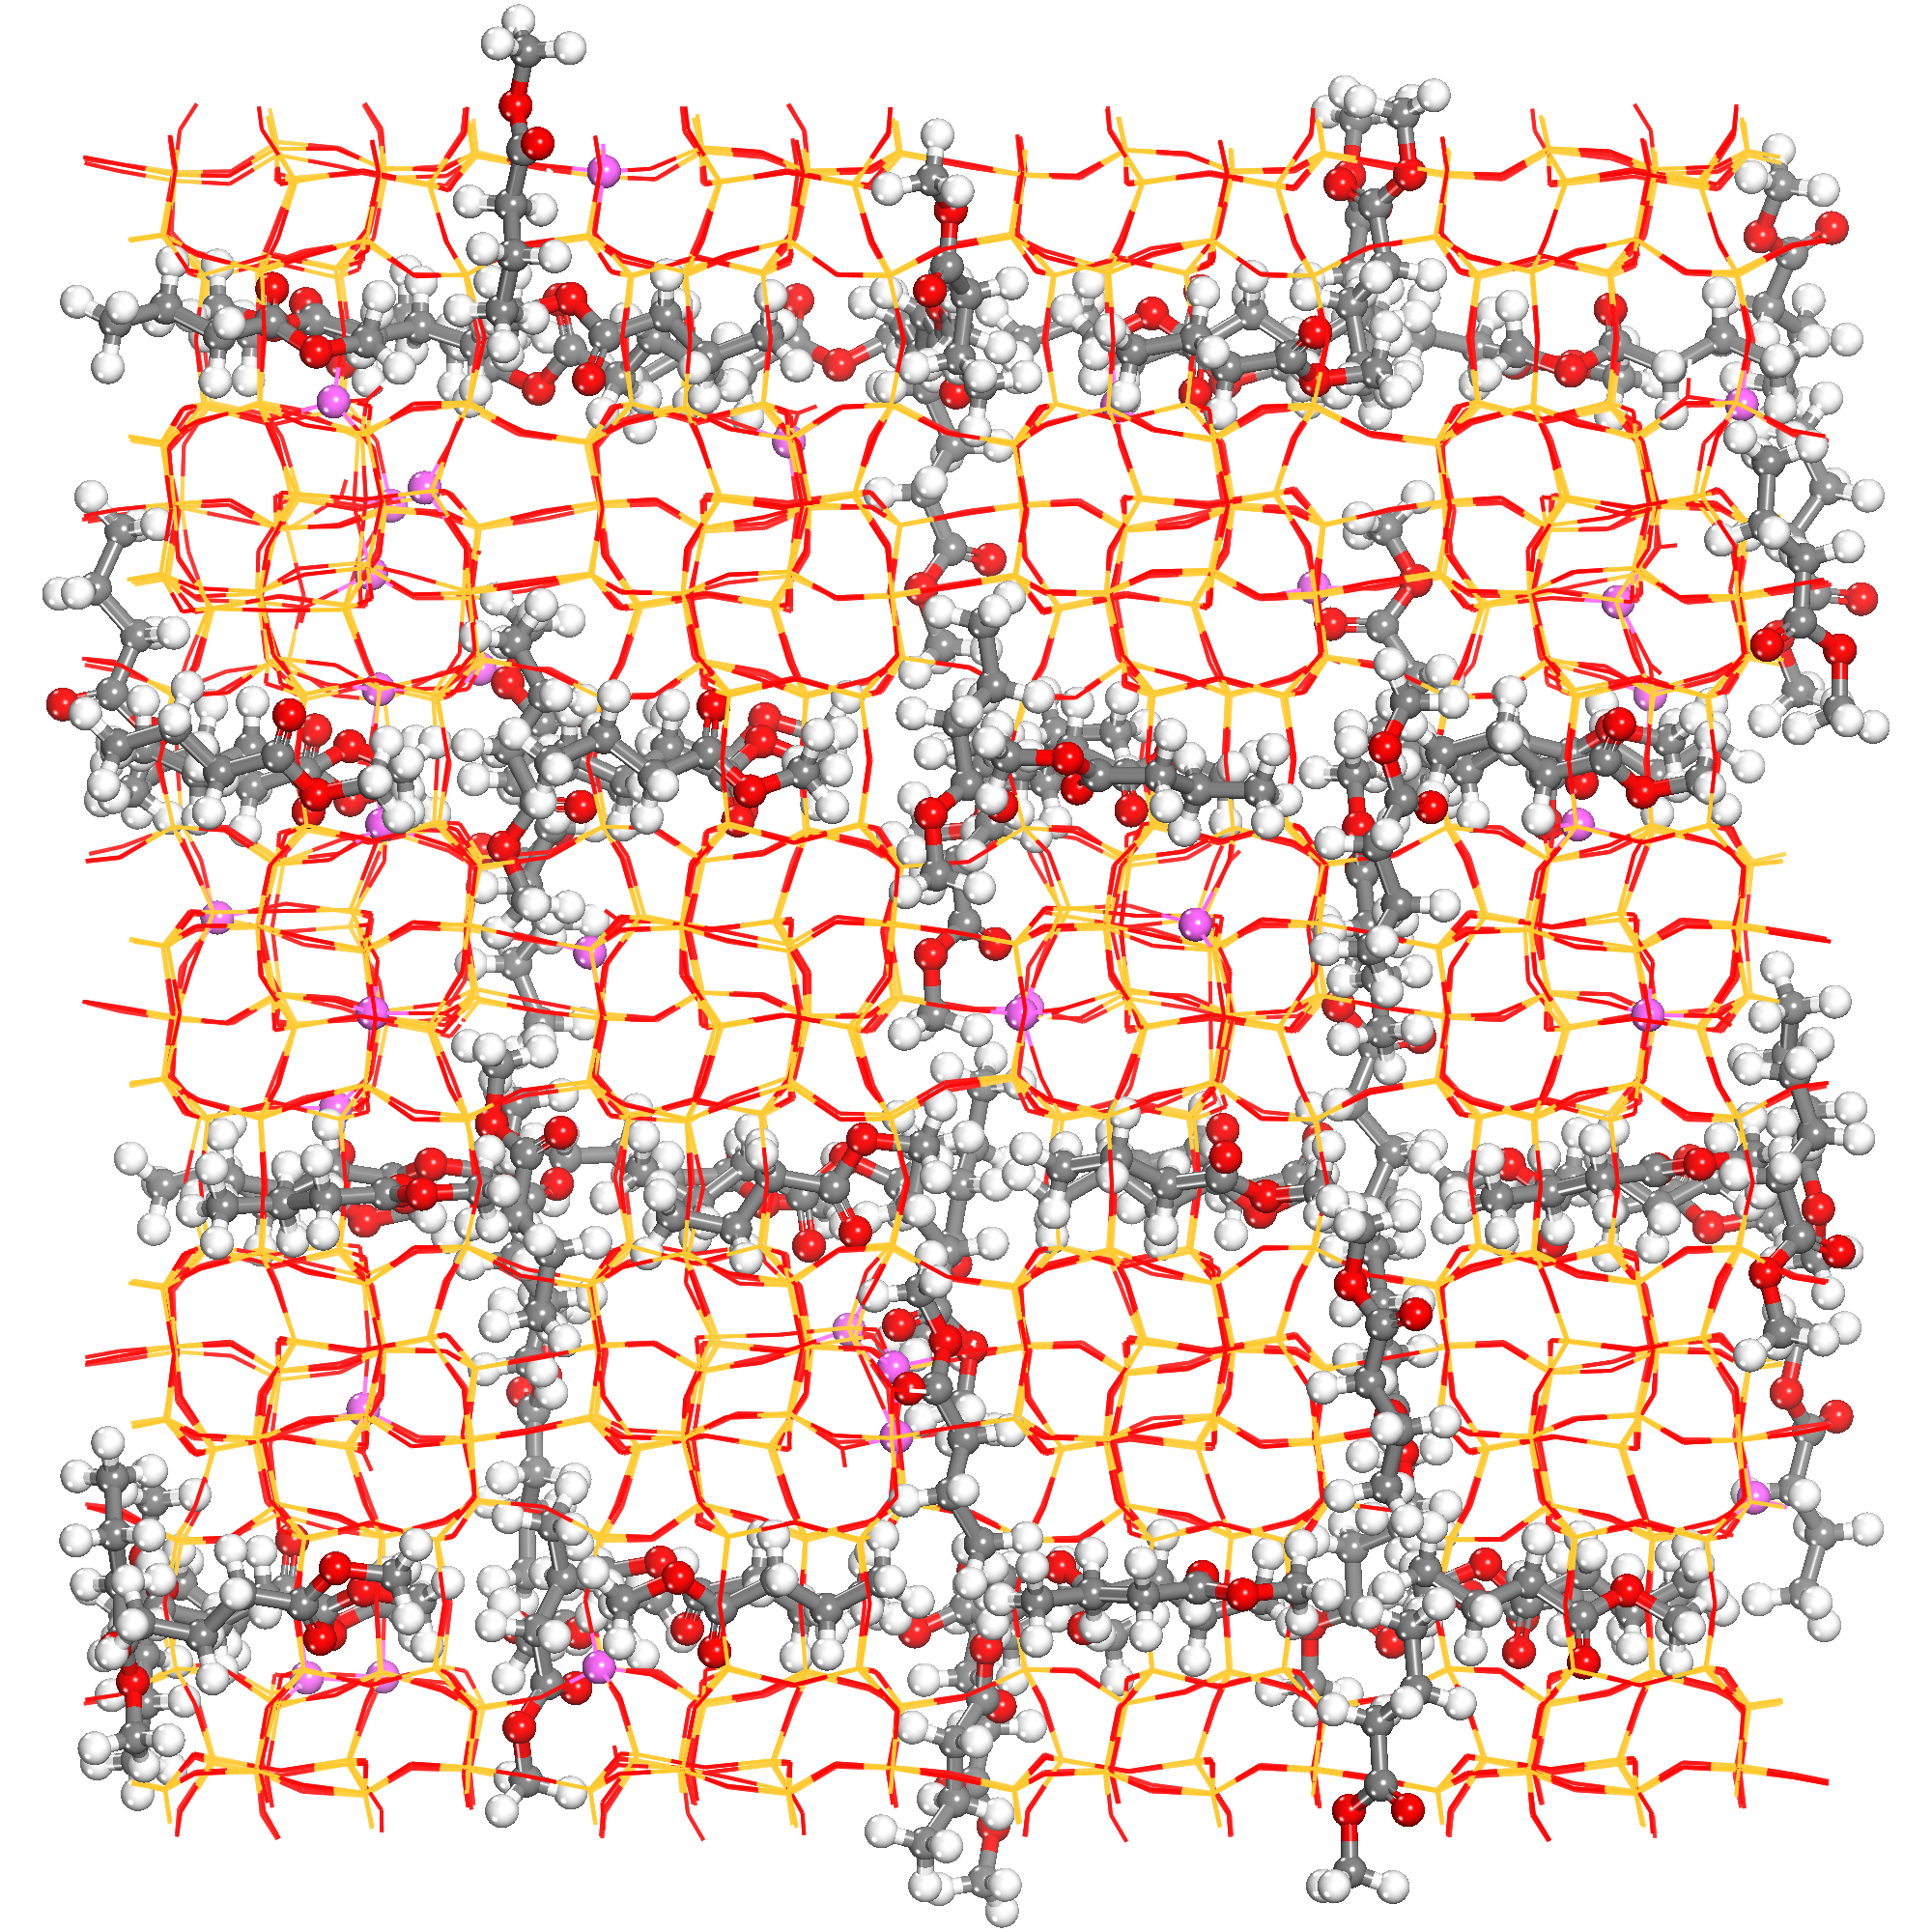
\includegraphics[width=1.8in]{figure/Adsorption/highC.png}
    %\caption{fig2}
    \end{minipage}%
    }%
    \caption{高低压力对丁酸甲酯吸附位置的构型对比图}
    \label{fig:loaction}
\end{figure}
\par{通过\reffig{fig:loaction}可以看出丁酸甲酯优先吸附在活性吸附位(B 位酸)处,并分布在交叉孔道旁,随着压力的增大,丁酸甲酯在交叉孔道和直孔道都有吸附,这与上文的结论是一致的,先吸附活性吸附位,再吸附一般吸附位。而通过\reffig{fig:L1}可以清楚地看到,丁酸甲酯中的双键氧与分子筛上的桥键氧上的氢(B位酸)形成了氢键。因为氢键的作用力比范德华力大,所以丁酸甲酯附着在活性吸附位放出的热量比一般吸附位大。从\reffig{fig:L2}可以看出,丁烯酸甲酯的双键与分子筛的B酸位相互作用形成 π 配位超分子复合物\cite{C-2-C-5直链烯烃在HY和H-ZSM-5分子筛上的吸附},使得丁烯酸甲酯与分子筛之间的作用力变强,从而丁烯酸甲酯的饱和吸附量更大,吸附平衡常数更大,这与上文的结论一致。}
% \begin{figure}[H]
%     \centering
%         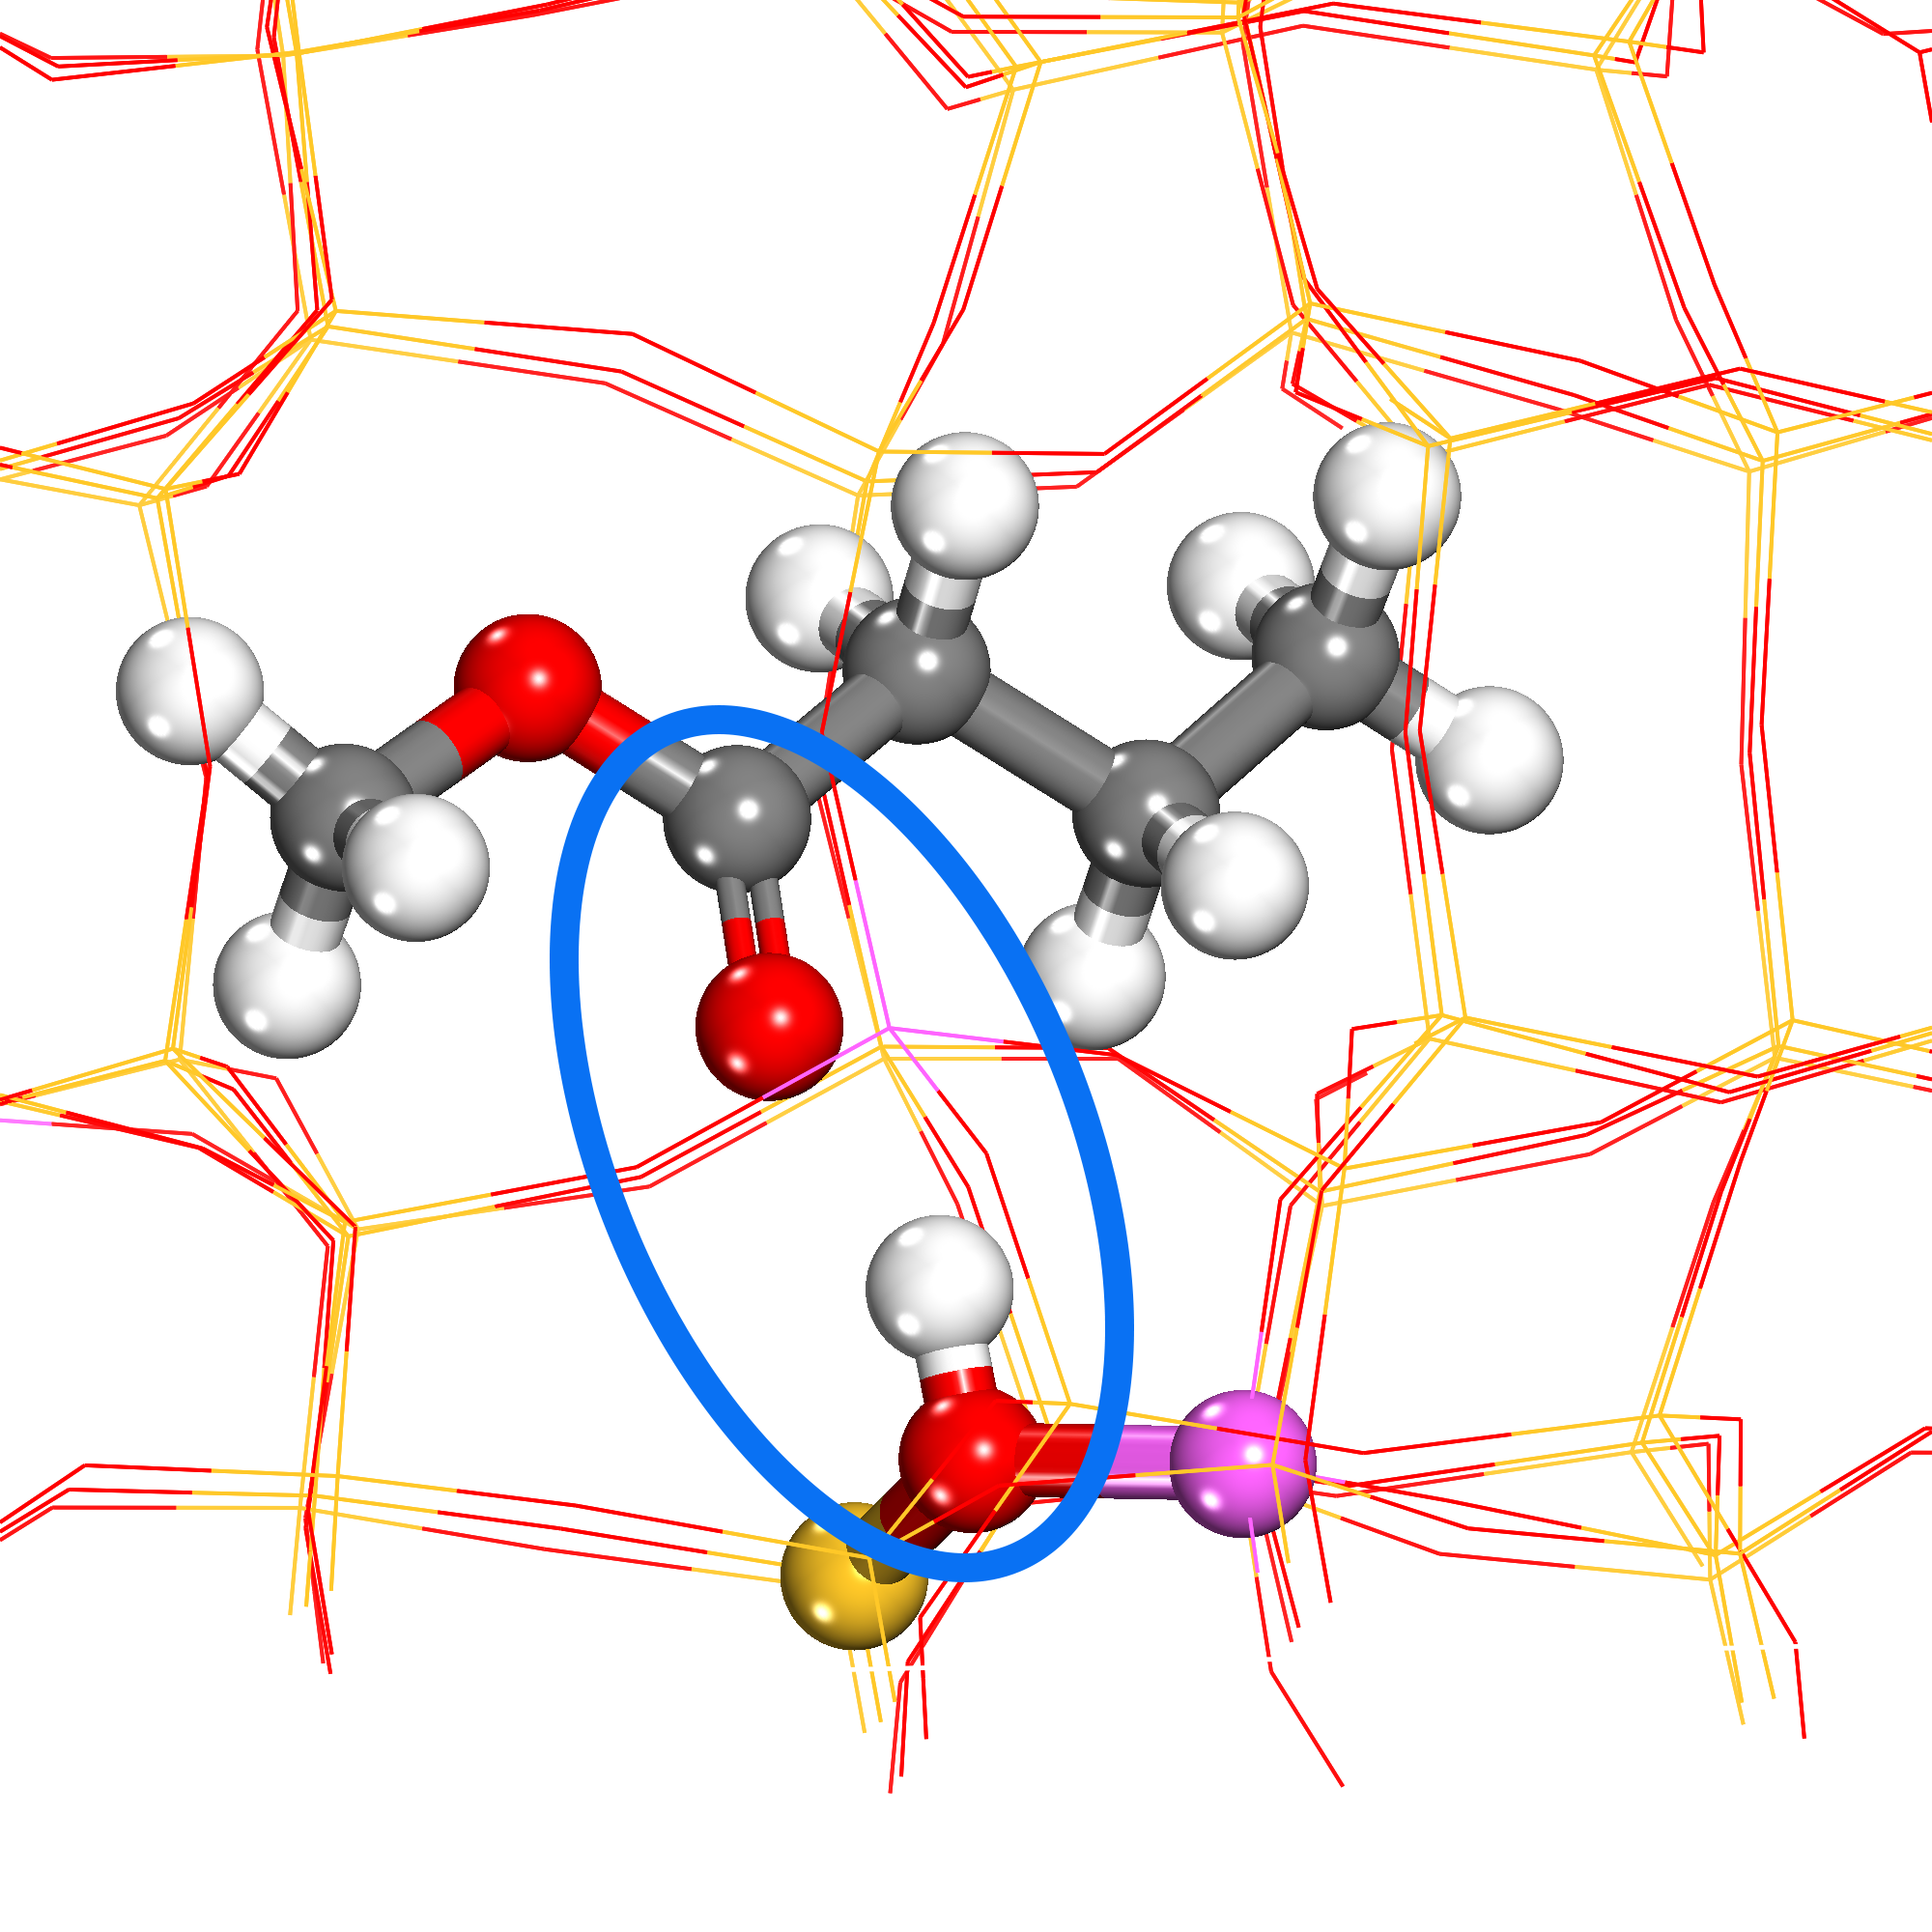
\includegraphics[width=0.5\textwidth]{figure/Adsorption/loaction.png}
%     \caption{丁酸甲酯与B位酸吸附构型图}
%     \label{fig:L}
% \end{figure}
% \par{为了讨论双键对吸附位的影响,进行丁酸甲酯在H-ZSM-5分子筛中的吸附构型模拟,结果如\reffig{fig:L1}所示}

% \begin{figure}[H]
%     \centering
%         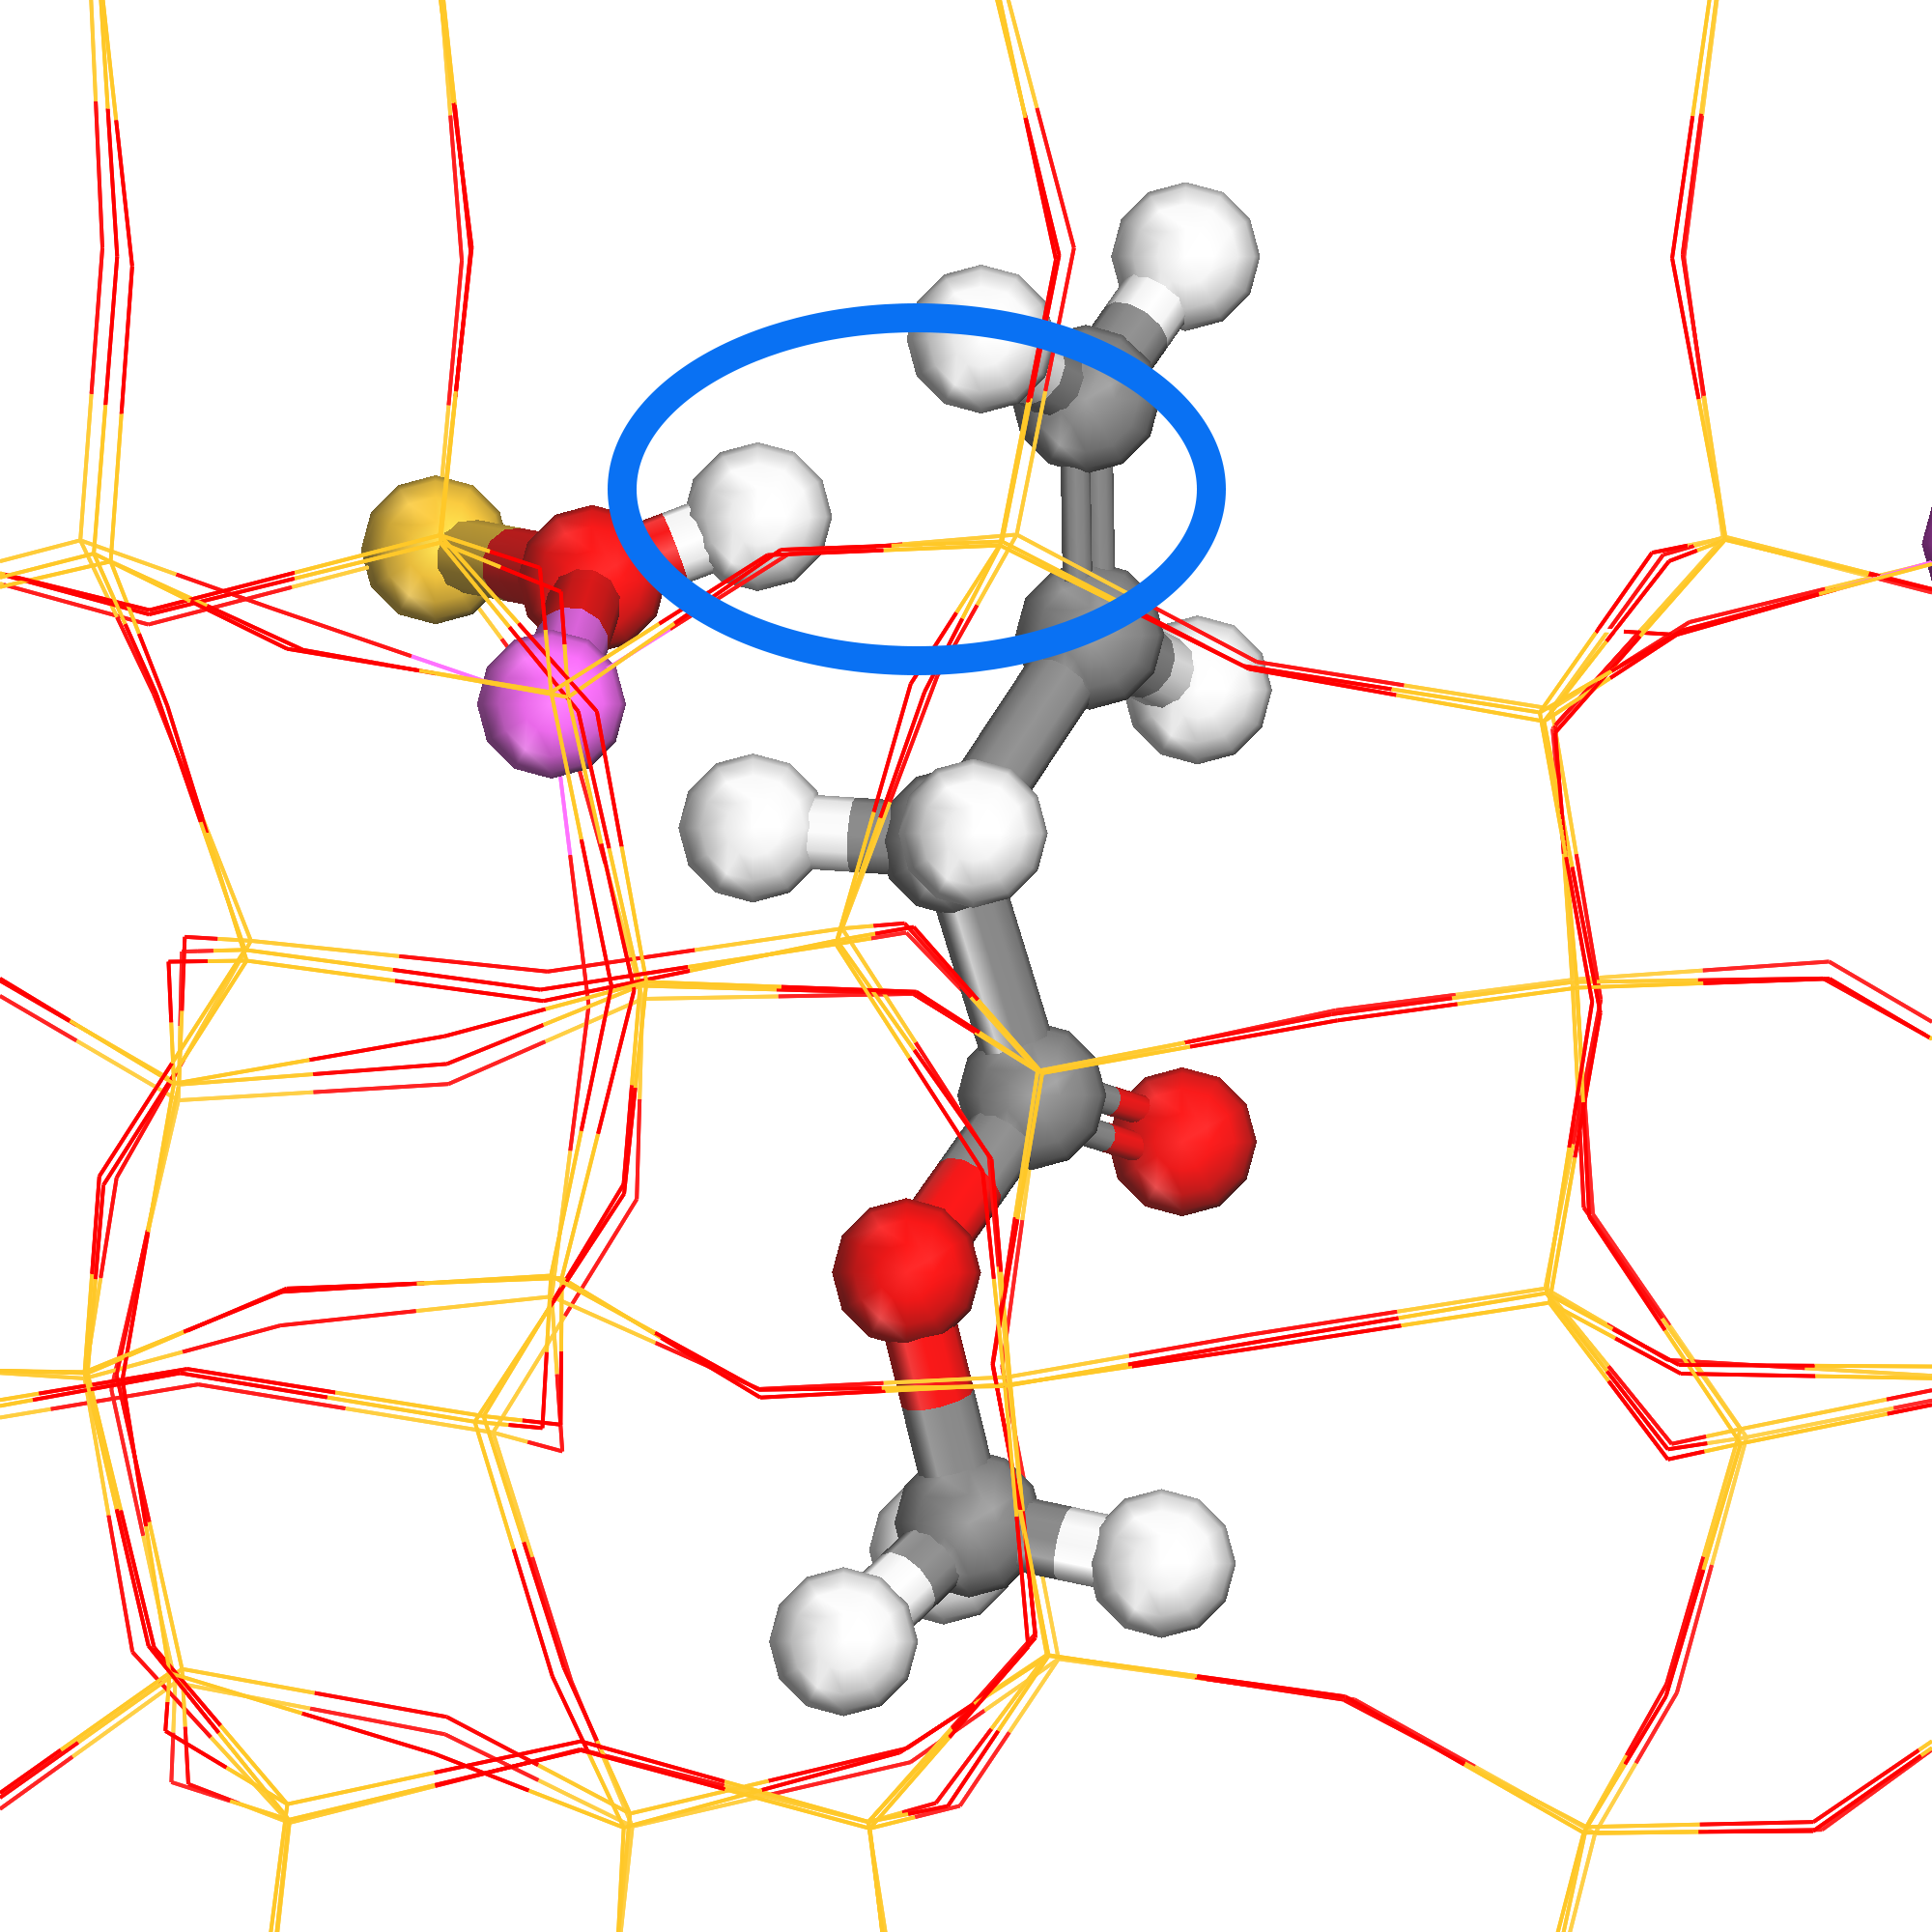
\includegraphics[width=0.5\textwidth]{figure/Adsorption/555.png}
%     \caption{丁烯酸甲酯与B位酸吸附构型图}
%     \label{fig:L1}
% \end{figure}
% \par{从\reffig{fig:L1}可以看出,丁烯酸甲酯的双键与分子筛的B酸位相互作用形成 π 配位超分子复合物\cite{C-2-C-5直链烯烃在HY和H-ZSM-5分子筛上的吸附},使得丁烯酸甲酯与分子筛之间的作用力变强,从而丁烯酸甲酯的饱和吸附量更大,吸附平衡常数更大,这与上文的结论一致。}

\begin{figure}[H]
    \centering

    \subfigure[丁酸甲酯与B位酸吸附构型图]{
    \begin{minipage}[t]{0.5\linewidth}
    \centering
    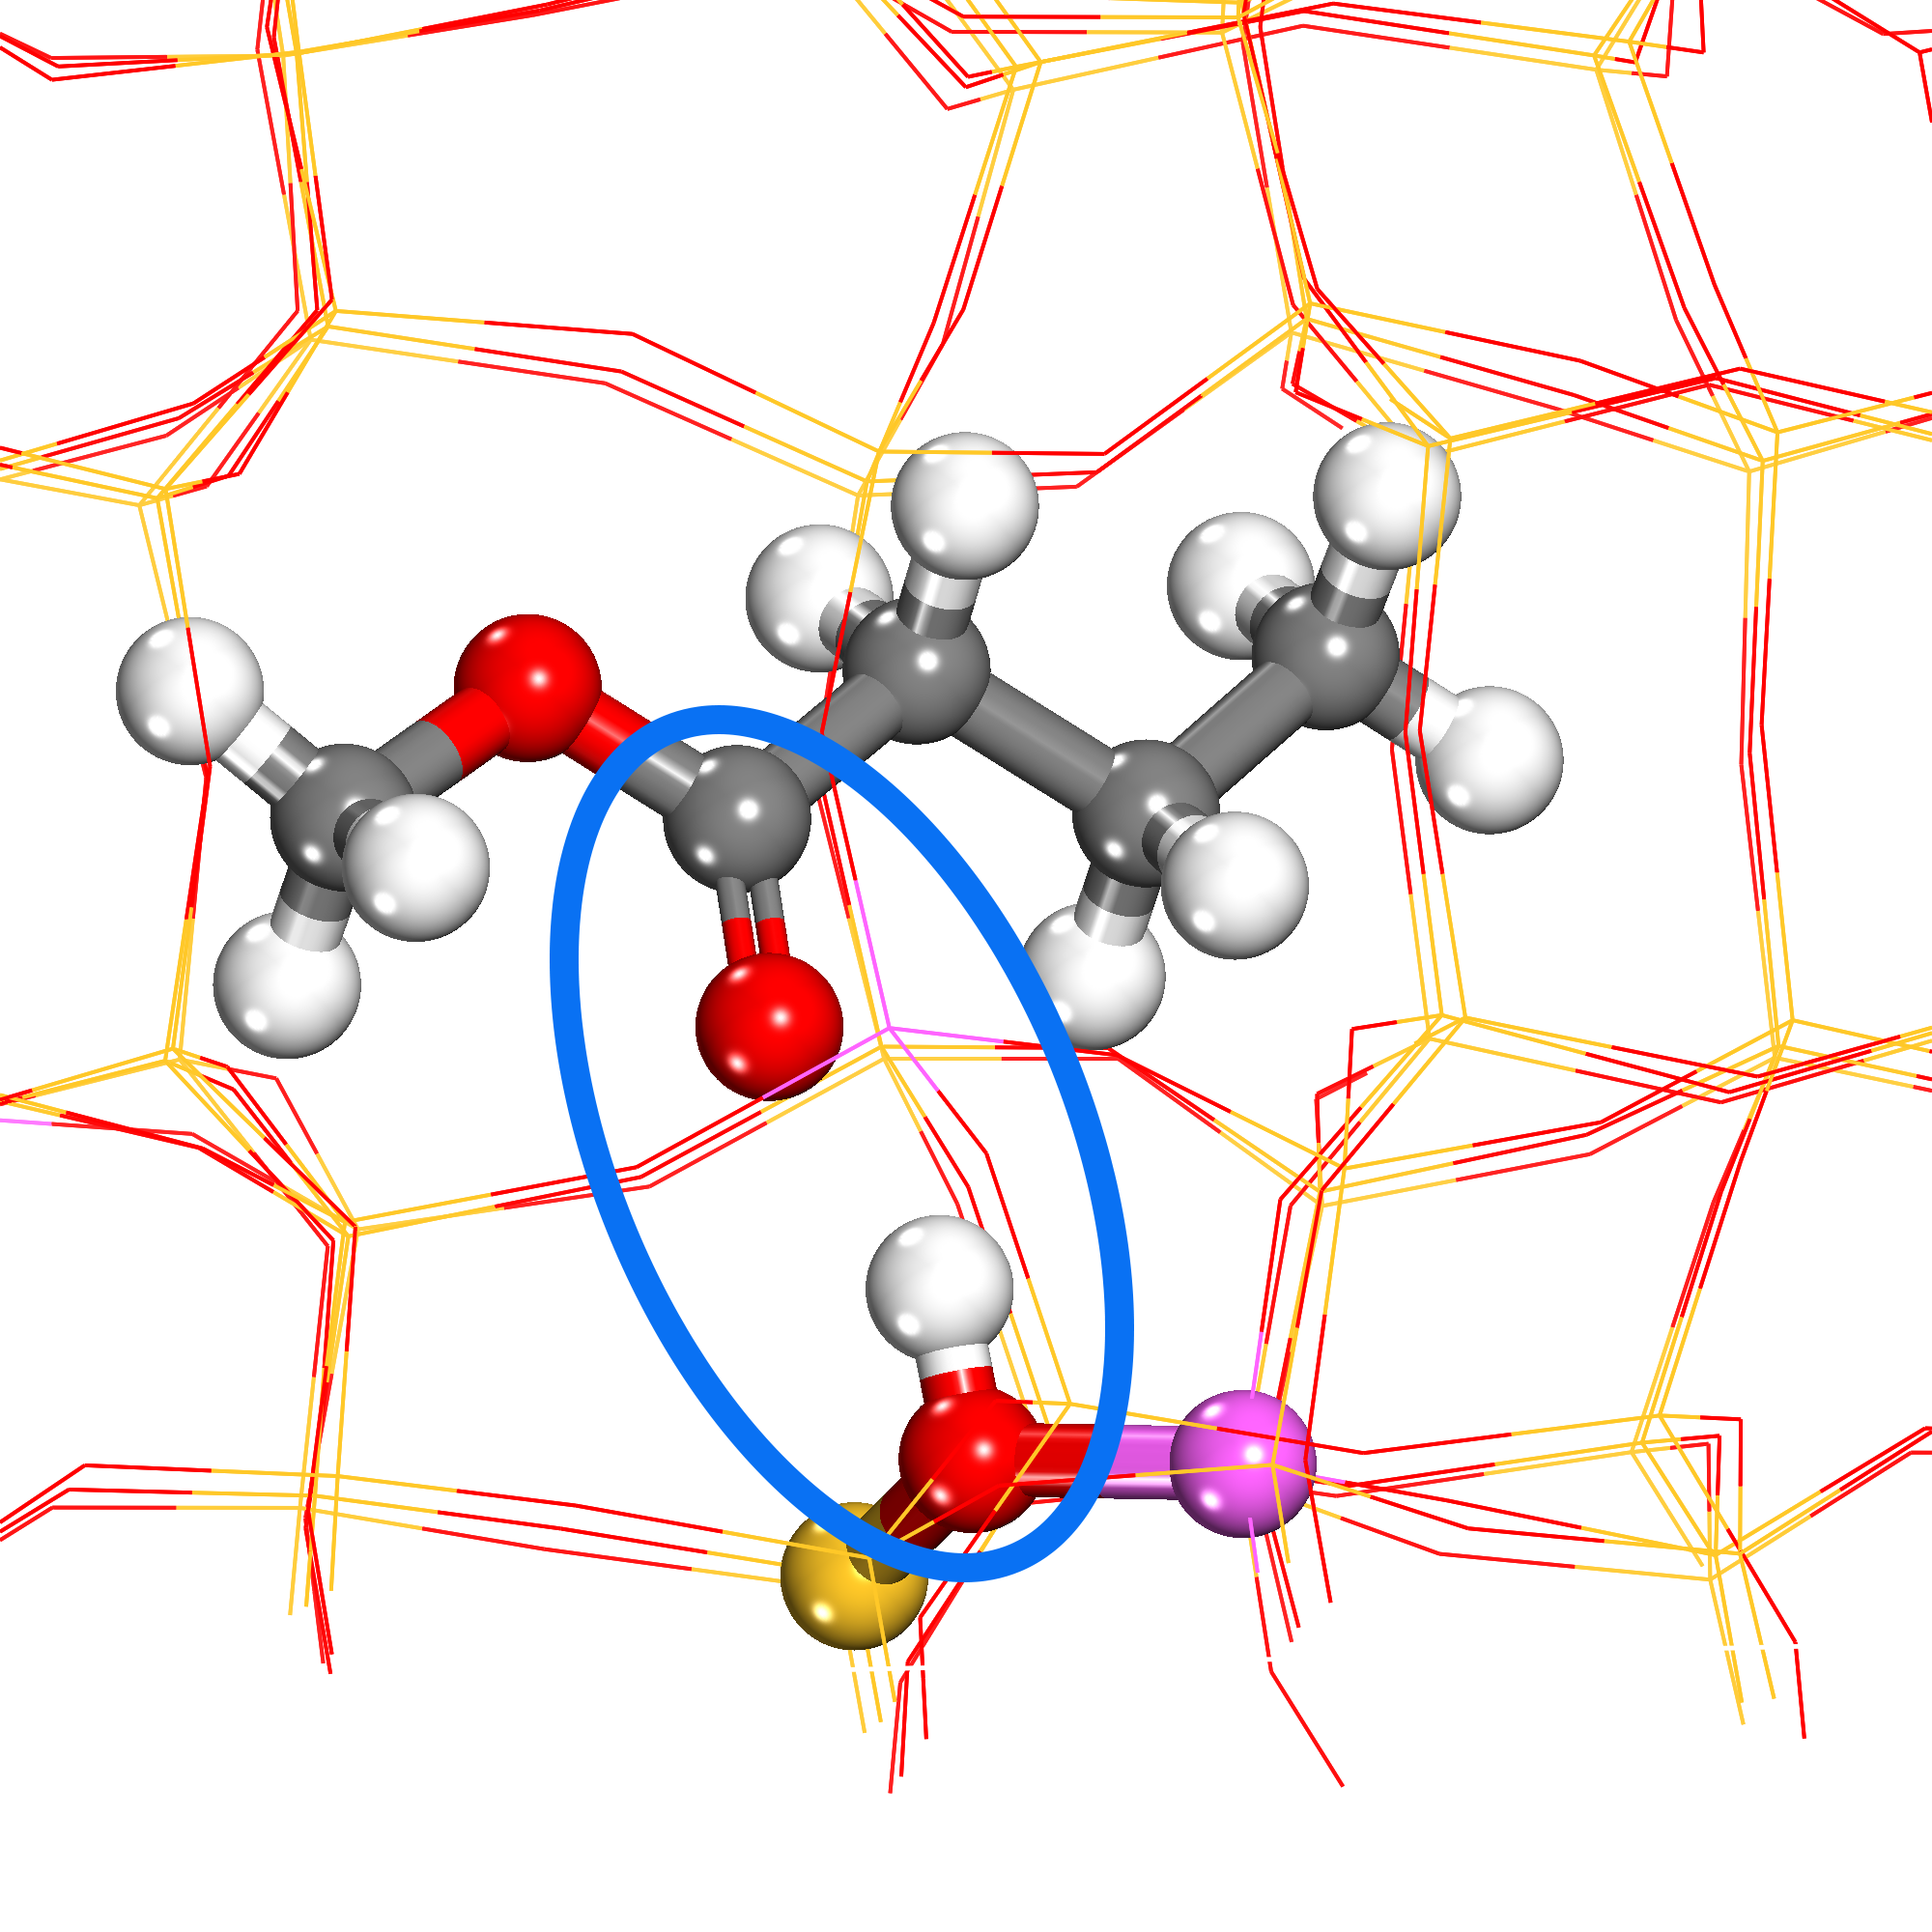
\includegraphics[width=2.7in]{figure/Adsorption/loaction.png}
    %\caption{fig1}
    \label{fig:L1}
    \end{minipage}%
    }%
    \subfigure[丁烯酸甲酯与B位酸吸附构型图]{
    \begin{minipage}[t]{0.5\linewidth}
    \centering
    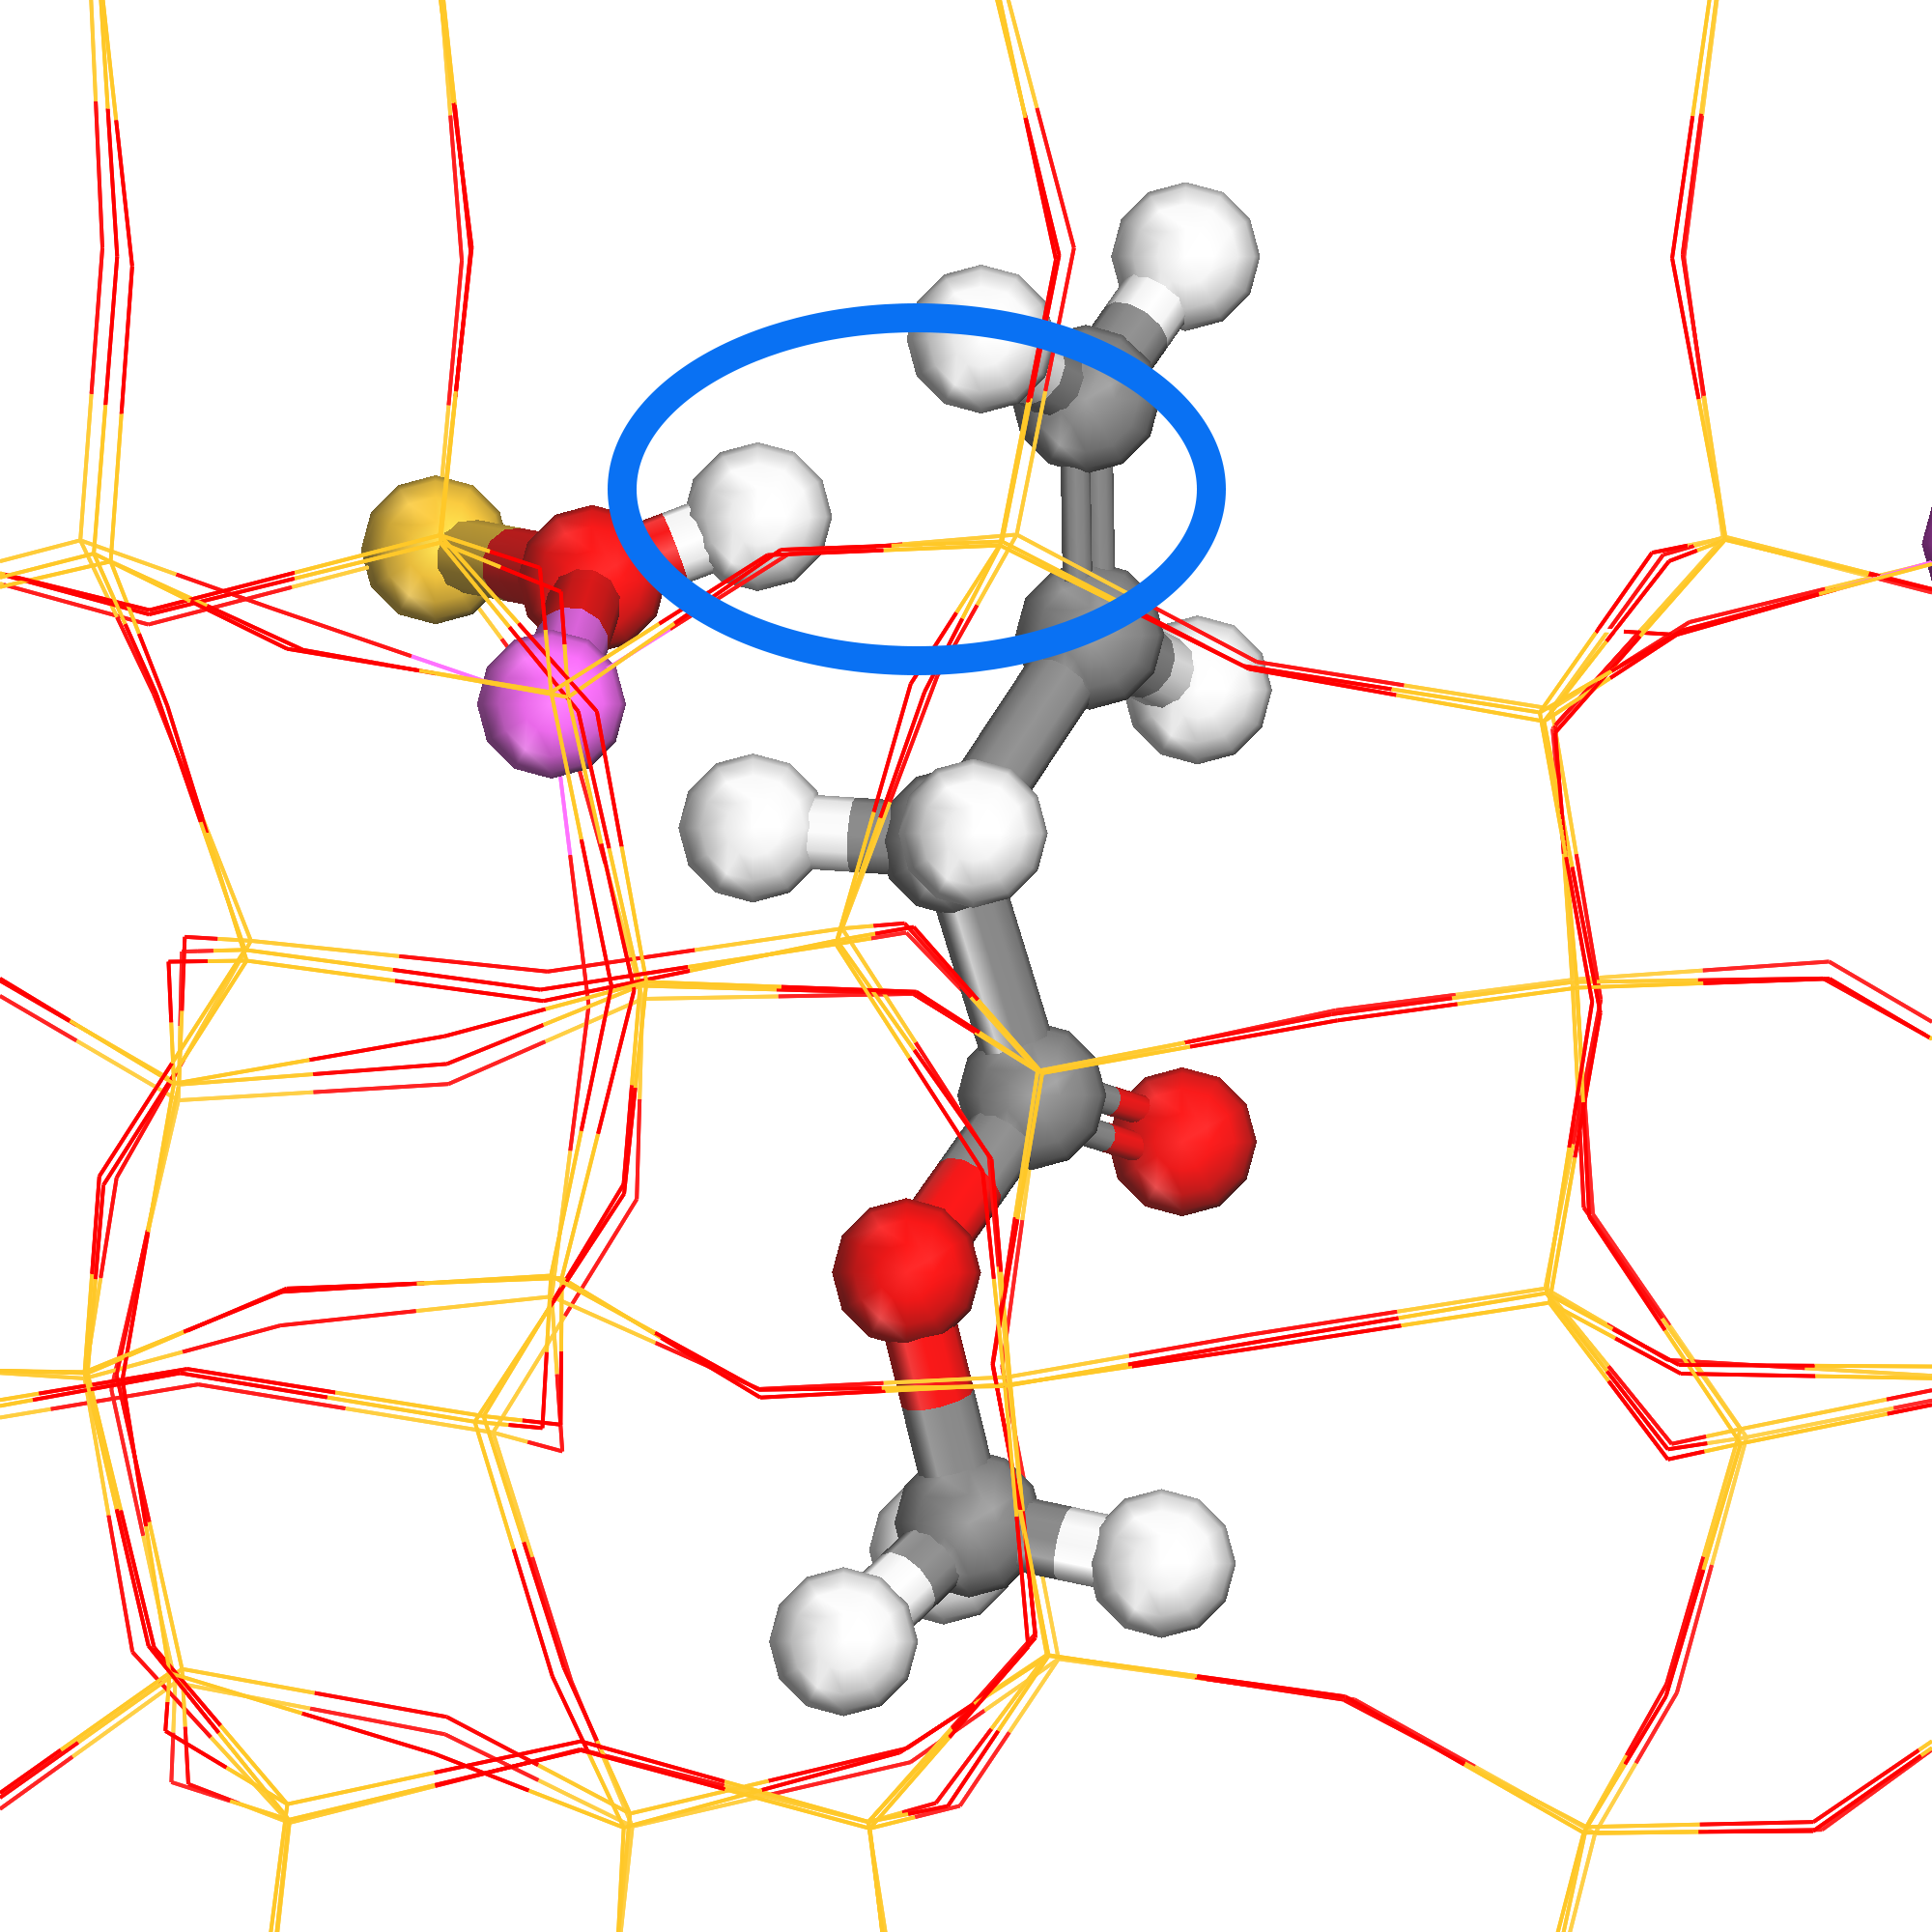
\includegraphics[width=2.7in]{figure/Adsorption/555.png}
    %\caption{fig2}
    \label{fig:L2}
    \end{minipage}%
    }%
    \caption{丁酸甲酯和丁烯酸甲酯与B位酸吸附构型图}
    \label{fig:L}
\end{figure}


\subsection{本章小结}
\par{本章采用GCMC(巨正则蒙特卡洛法),通过Materials Studio 8.0软件中的Sorption模块对丁酸甲酯等模型化合物在H-ZSM-5分子筛中进行了吸附模拟,得到以下结论:}
\begin{enumerate}
    \item 丁酸甲酯等模型化合物在微介孔H-ZSM-5分子筛的吸附等温线均属于\RNum{1}型等温线。随着孔径的增大,饱和吸附量减小,吸附平衡常数减小,单位质量分子筛的饱和吸附量先增大后减小,20Å介孔最大;随着温度的增大,饱和吸附量减小,吸附平衡常数减小;随着吸附分子极性增强,饱和吸附量增大,吸附平衡常数增大;随着吸附分子链长的增大,饱和吸附量减小,吸附平衡常数增大。
    \item 丁酸甲酯在微孔和介孔中的等量吸附热随压力(吸附量)的变化不同:在微孔中,随着压力的增大,等量吸附热以增量逐渐减小的方式增大,最后趋于最大值,而随着吸附量的增大,等量吸附热线性增大;在介孔中,随着压力或吸附量的增大,等量吸附热先增大再减小,有一个极大值。随着孔径的增大,相同压力下的等量吸附热减小。随着温度的增加,微孔介孔的等量吸附热都减小,在介孔中的等量吸附热最大值对应的压力几乎不变。在介孔中,随着温度的增加,孔径越大,等量吸附热最大值所对应的吸附量变化越小。
    \item 通过吸附构型图,可以发现丁酸甲酯优先吸附在活性吸附位(B位酸)处,并分布在交叉孔道旁,B位酸与双键氧形成氢键,随着压力的增大,丁酸甲酯在交叉孔道和直孔道都有吸附。丁烯酸甲酯中的双键与B位酸形成 π 配位超分子复合物。
\end{enumerate}
